\documentclass[12pt]{beamer}
\usepackage{ucltemplate}


\usepackage{lineno,hyperref}
\usepackage{stfloats}
\usepackage{tikz} % Package for drawing
\usepackage{amsmath}
\usepackage{mathtools}
\usepackage{amsfonts}
\usepackage{float}
\usepackage{lmodern,bm}                
\usepackage[T1]{sansmath} 
\usepackage{amsthm}
\usepackage{url}
\usepackage[toc,page]{appendix}
\usepackage{graphicx}
\usepackage{subcaption}
\usepackage{verbatim} %to comment out sections
\usetikzlibrary{shapes.multipart}
\usetikzlibrary{matrix}
\usetikzlibrary{positioning}
\usepackage{float}
\usepackage{color}
\usepackage{booktabs}
\usepackage{placeins}
\usepackage{bm}
\usepackage[natbib=true,style=authoryear,backend=bibtex,useprefix=true]{biblatex}

\newcommand{\myfootnote}[1]{
    \renewcommand{\thefootnote}{}
    \footnotetext{\scriptsize#1}
    \renewcommand{\thefootnote}{\arabic{footnote}}
}
\setbeamerfont{footnote}{size=\tiny}
\addbibresource{bibliography.bib}

\newcommand{\curl}{\mathbf{curl}}
\newcommand{\divergence}{\textnormal{div}}
\DeclarePairedDelimiter\floor{\lfloor}{\rfloor}

\title{Fast Calder\'on preconditioning of the PMCHWT formulation for scattering by multiple dielectric objects}
\subtitle[The subtitle]{\tiny{$14^{th}$ International Conference on Mathematical and Numerical Aspects of Wave Propagation, Vienna, Austria}}
\author{\textbf{Antigoni Kleanthous} \inst{1},  Timo Betcke \inst{1}, David Hewett \inst{1}, Carlos Jerez-Hanckes \inst{2}, Paul Escapil-Inchausp\'e \inst{3}, Anthony J. Baran \inst{4,5}}
\institute{\inst{1} Department of Mathematics, UCL, UK  \\ \inst{2} Universidad Adolfo Iba\~nez, Santiago, Chile \\
\inst{3} Pontificia Universidad Cat\'olica de Chile, Santiago, Chile \\
\inst{4} Met Office, UK \\ \inst{5} School of Physics, Astronomy, and Mathematics, University of Hertfordshire, UK}
\date{30 August 2019}

\usepackage{pdfpages}

\begin{document}
\begin{frame}

\includepdf{Figures/PostgradSeminar_title_slide.pdf}
\end{frame}

%%%
\begin{frame}{Introduction}
\myfootnote{\fullcite{kleanthous2019calderon}} 
Plan
\begin{itemize}
\item Motivation: Ice Crystals in cirrus clouds
\item The scattering problem
\item Boundary Integral Operators
\item The PMCHWT formulation
\item Discretisation
\item Calder\'on Preconditioning
\item Benchmarks and numerical examples using BEMPP (\url{www.bempp.com})
\item Accelerated Calder\'on preconditioning
\item More numerical examples
\item Met Office work
\end{itemize}
\end{frame}
%%%

%%%%
\begin{frame}{Motivation: Ice Crystals in cirrus clouds}
\myfootnote{\fullcite{baran2012single}}
\centering
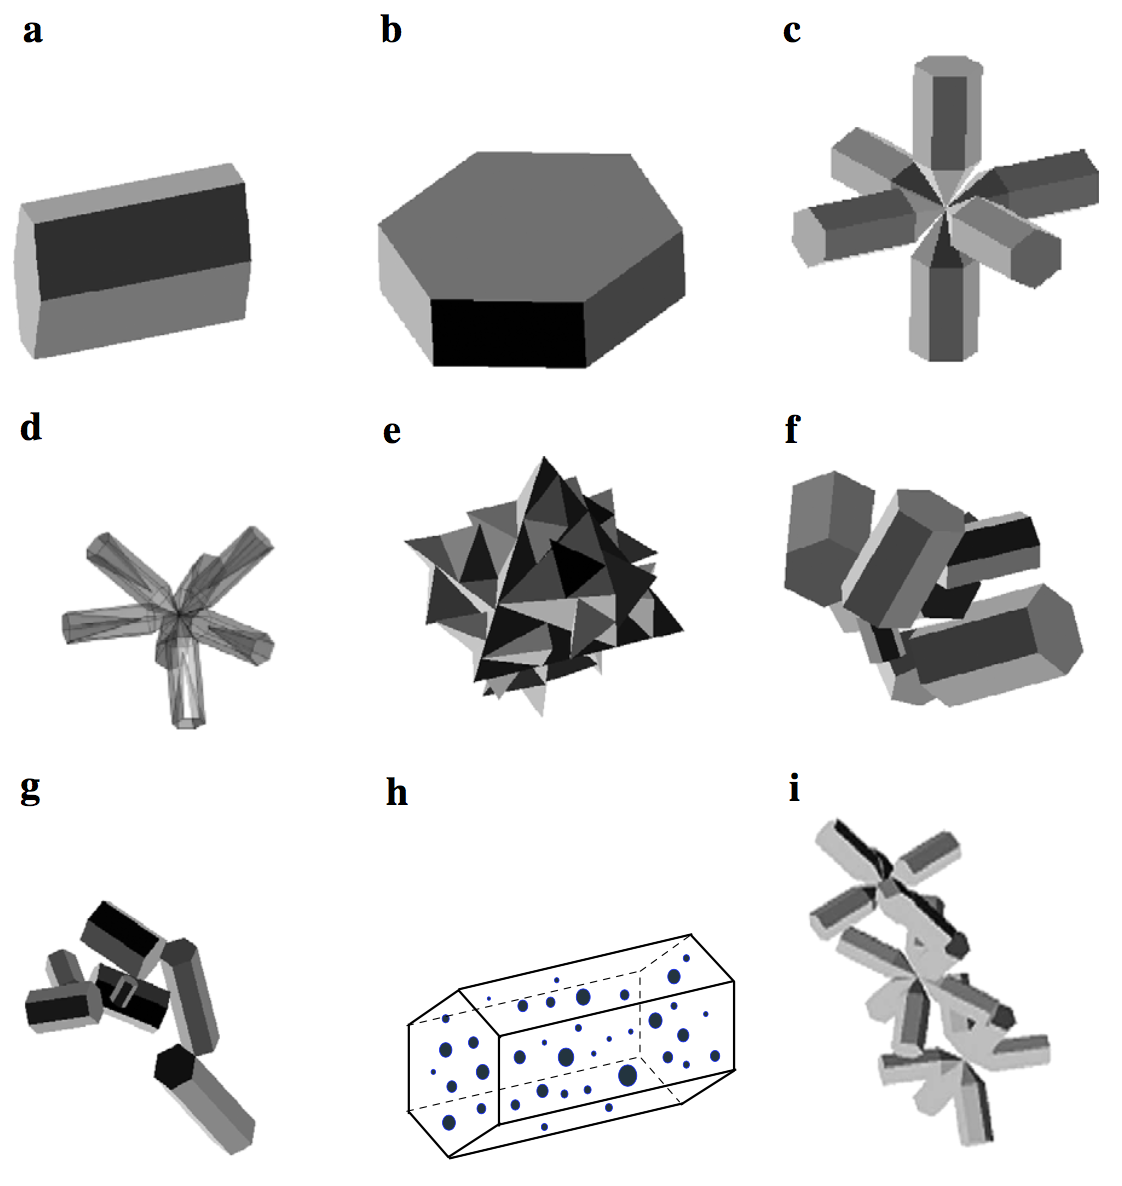
\includegraphics[width = 0.6 \textwidth]{Figures/ice_crystals.png}
    
\end{frame}

%%%
\begin{frame}{The scattering problem}
\vspace{0.2cm}
\centering
    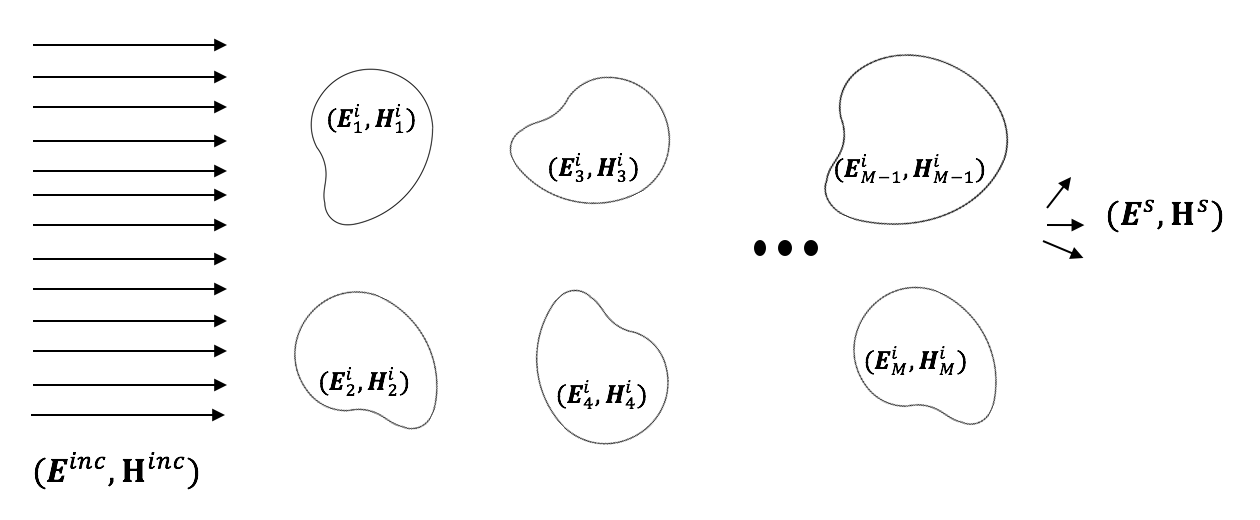
\includegraphics[width = \textwidth]{Figures/problem.png}
    
\vspace*{-0.5cm}    
\begin{footnotesize}    
\begin{itemize}
    \item $(\mathbf{E}^i_m, \mathbf{H}^i_m)$ and $(\mathbf{E}^e, \mathbf{H}^e)$: interior and exterior fields with
        \begin{alignat}{1}
            \mathbf{E}^e = \mathbf{E}^{inc} + \mathbf{E}^s, \quad 
            \mathbf{H}^e = \mathbf{H}^{inc} + \mathbf{H}^s, \nonumber
        \end{alignat}
    \item Time-harmonic Maxwell equations
    \begin{alignat}{3}
        \only<1>{\nabla \times \mathbf{E}^i_m &=& i \omega \mu_m \mathbf{H}^i_m, \quad \nabla \times \mathbf{H}^i_m &=& - i \omega \epsilon_m \mathbf{E}^i_m, &\qquad\text{in }\Omega^i_m, \nonumber \\
        \nabla \times \mathbf{E}^e &=& i \omega \mu_e \mathbf{H}^e, \quad \nabla \times \mathbf{H}^e &=& - i \omega \epsilon_e \mathbf{E}^e &\qquad\text{in }\Omega^e, \nonumber}
        \only<2>{&\nabla \times (\nabla \times \mathbf{E}^i_m) &-& k_m^2 \mathbf{E}^i_m &= 0,\qquad&\text{in }\Omega^i_m, \nonumber\\
        &\nabla \times (\nabla \times \mathbf{E}^e) &-& k_e^2 \mathbf{E}^e &= 0,\qquad&\text{in }\Omega^e, \nonumber} 
\end{alignat}
    \item Transmission boundary conditions
        \begin{alignat}{3}
            \only<1>{\mathbf{E}^i_m (\mathbf{x}) \times \mathbf{n} &= \mathbf{E}^e (\mathbf{x}) \times \mathbf{n}, \quad \mathbf{H}^i_m (\mathbf{x}) \times \mathbf{n} &= \mathbf{H}^e (\mathbf{x}) \times \mathbf{n}, && \quad \mathbf{x} \in \Gamma_m. \nonumber}
            \only<2>{\mathbf{E}^i_m (\mathbf{x}) \times \mathbf{n} &= \mathbf{E}^e (\mathbf{x}) \times \mathbf{n}, && \quad \mathbf{x} \in \Gamma_m. \nonumber}
\end{alignat}
\end{itemize}
\end{footnotesize}
\end{frame}
%%%

% %%%
% \begin{frame}{Function Spaces}
% \myfootnote{\fullcite{buffa2003galerkin}}
% \small{
% \begin{itemize}
% \item  \textcolor{bluecolour}{Tangential Trace Space}: $\mathbf{H}_\times^{\frac{1}{2}} (\Gamma) = \{ \gamma_D^- \mathbf{u} : \mathbf{u} \in \mathbf{H}^1(\Omega _i)\}$

% Dual: $\mathbf{H}_\times^{-\frac{1}{2}} (\Gamma)$ w.r.t $\langle \mathbf{u}\mathbf{v}\rangle _\tau = \int _\Gamma \mathbf{u} \cdot (\mathbf{n} \times \mathbf{v}) d\Gamma$
% %
% \item Space of \textcolor{bluecolour}{surface div-conforming functions}:
% \begin{eqnarray}
% \mathbf{H}_\times^{-\frac{1}{2}} (\textnormal{div}_\Gamma, \Gamma) = \{ \mathbf{u} \in \mathbf{H}_\times^{-\frac{1}{2}} (\Gamma) : \textnormal{div}_\Gamma \mathbf{u} \in \mathbf{H}^{-\frac{1}{2}} (\Gamma) \} \nonumber
% \end{eqnarray}
% %
% \item Space of \textcolor{bluecolour}{surface curl-conforming functions}:
% \begin{eqnarray}
% \mathbf{H}_\times^{-\frac{1}{2}} (\textnormal{curl}_\Gamma, \Gamma) = \{ \mathbf{n} \times \mathbf{u} : \mathbf{u} \in \mathbf{H}_\times^{-\frac{1}{2}} (\textnormal{div}_\Gamma, \Gamma) \} \nonumber
% \end{eqnarray}
% \end{itemize}
% }
% \end{frame}
% %%

%%%
\begin{frame}{Boundary Integral Operators}
\begin{footnotesize}
    \begin{itemize}
        \item Electric and Magnetic Potential Operators
            \begin{alignat}{2}
                &\mathcal{E} \mathbf{v}(\mathbf{x}) &:=& ik \int _{\Gamma} \mathbf{v}(\mathbf{y}) G (\mathbf{x}, \mathbf{y}) d \Gamma (\mathbf{y}) - \frac{1}{ik} \nabla_\mathbf{x} \int _\Gamma \nabla_\mathbf{y} \cdot \mathbf{v}(\mathbf{y}) G (\mathbf{x}, \mathbf{y}) d\Gamma (\mathbf{y}), \nonumber\\
                %
                &\mathcal{H} \mathbf{v}(\mathbf{x}) &:=& \nabla_\mathbf{x} \times \int _\Gamma \mathbf{v}(\mathbf{y}) G (\mathbf{x}, \mathbf{y}) d \Gamma (\mathbf{y}), \nonumber 
            \end{alignat}
            where $G (x,y) = \frac{\exp (ik | \mathbf{x} - \mathbf{y}|)}{4 \pi | \mathbf{x} - \mathbf{y}|}$
        \item Dirichlet and Neumann Traces
            \begin{alignat}{3}
                \gamma_{D}^{\pm} \mathbf{u} (\mathbf{x}) &:= \mathbf{u}(\mathbf{x}) \times \mathbf{n}, \quad 
                \gamma_{N}^{\pm} \mathbf{u}(\mathbf{x}) &:= \frac{1}{ik} \gamma_{D}^{\pm} \left( \nabla \times \mathbf{u}(\mathbf{x}) \right), \quad &\mathbf{x} \in \Gamma \nonumber 
            \end{alignat}
        \item Boundary Integral Operators
            \begin{alignat}{3}
                &\mathcal{S} &:=& \{ \gamma_D \}\mathcal{E} &=& -\{ \gamma_{N} \} \mathcal{H}, \nonumber \\
                &\mathcal{C} &:=& \{ \gamma _{D} \} \mathcal{H} &=& \{ \gamma _{N} \} \mathcal{E}, \nonumber 
            \end{alignat}
    \end{itemize}
\end{footnotesize}
\end{frame}
%%%

%%%
\begin{frame}{Boundary Integral Operators}
\begin{footnotesize}
\begin{itemize}
    \item Stratton Chu Representation Formulae
        \begin{alignat}{3}
            \mathcal{H}^i_m (\gamma_{D,m}^- \mathbf{E}^i_m) &+ \mathcal{E}^i_m (\gamma_{N,m}^- \mathbf{E}^i_m) &= 
            \begin{cases}
                \mathbf{E}^i_m(\mathbf{x}), & \mathbf{x} \in \Omega^i_m, \\
                \mathbf{0}, & \mathbf{x} \not \in \overline{\Omega^i_m},
            \end{cases} \nonumber\\
            %
            -\sum_m^M \mathcal{H}^e_m (\gamma_{D,m}^+ \mathbf{E}^s) &- \sum_m^M  \mathcal{E}^e_m (\gamma_{N,m}^+ \mathbf{E}^s) &= 
            \begin{cases}
                \mathbf{E}^s(\mathbf{x}), & \mathbf{x} \in \Omega_e, \\
                \mathbf{0}, & \mathbf{x} \not \in \overline{\Omega_e},
            \end{cases} \nonumber 
        \end{alignat}
\end{itemize}
\end{footnotesize}    
\end{frame}
%%%

% %%%
% \begin{frame}{Boundary Integral Operators}
% \begin{footnotesize}
% Taking appropriate interior and exterior Dirichlet and Neumann traces of the Stratton Chu representation formulae
% \begin{align}
% &\left( \frac{1}{2}\bm{\mathcal{I}}_m - \bm{\mathcal{{A}}}^i_m \right){\mathbf{u}}^i_m = 0, \nonumber\\
% &\left( \frac{1}{2} \bm{\mathcal{I}}_m + \bm{\mathcal{{A}}}^e_m \right) {\mathbf{u}}^s_m + \sum _{\ell \neq m}^M \bm{\mathcal{{A}}}_{m\ell} {\mathbf{u}}^s_\ell= 0 , \nonumber 
% \end{align}
% where
% \begin{gather}
% \bm{\mathcal{{A}}}^i_m = \begin{bmatrix}
% \mathcal{C}^i_m & \frac{\mu_m}{k_m} \mathcal{S}^i_m \\[6pt]
% -\frac{k_m}{\mu_m} \mathcal{S}^i_m & \mathcal{C}^i_m
% \end{bmatrix}, \quad 
% \bm{\mathcal{{A}}}^e_m = \begin{bmatrix}
% \mathcal{C}^e_m & \frac{\mu_e}{k_e} \mathcal{S}^e_m \\[6pt]
% -\frac{k_e}{\mu_e} \mathcal{S}^e_m & \mathcal{C}^e_m
% \end{bmatrix}, \nonumber \\
% \bm{\mathcal{{A}}}_{m\ell} = \begin{bmatrix}
%     \mathcal{C}^e_{m\ell} & \frac{\mu_e}{k_e} \mathcal{S}^e_{m\ell} \\[6pt]
%     -\frac{k_e}{\mu_e} \mathcal{S}^e_{m\ell} & \mathcal{C}^e_{m\ell}
% \end{bmatrix}, \quad
% %
% {\mathbf{u}}^i_m = \begin{bmatrix}
%     \gamma_{D,m}^{-} \mathbf{E}^i_m \\[6pt]
%     \frac{k_m}{\mu_m} \gamma_{N,m}^- \mathbf{E}^i_m
% \end{bmatrix}, \quad 
% %
% {\mathbf{u}}^s_m = \begin{bmatrix}
%     \gamma_{D,m}^+ \mathbf{E}^s \\[6pt]
%     \frac{k_e}{\mu_e} \gamma_{N,m}^+ \mathbf{E}^s
% \end{bmatrix} \nonumber .
% \end{gather}
% \end{footnotesize}    
% \end{frame}
% %%%

% %%%
% \begin{frame}{The PMCHWT formulation}
% \begin{footnotesize}
% Combine
% \begin{align}
% &\left( \frac{1}{2}\bm{\mathcal{I}}_m - \bm{\mathcal{{A}}}^i_m \right){\mathbf{u}}^i_m = 0, \nonumber\\
% &\left( \frac{1}{2} \bm{\mathcal{I}}_m + \bm{\mathcal{{A}}}^e_m \right) {\mathbf{u}}^s_m + \sum _{\ell \neq m}^M \bm{\mathcal{{A}}}_{m\ell} {\mathbf{u}}^s_\ell= 0 , \nonumber 
% \end{align}
% with transmission conditions
% \begin{alignat}{3}
% {\mathbf{u}}^i_m = {\mathbf{u}}^s_m + {\mathbf{u}}^{inc}_m,\quad m=1,\ldots, M, \nonumber
% \end{alignat}
% to get the PMCHWT formulation for each $m$
% \begin{alignat}{1}
% \left(\bm{\mathcal{{A}}}^i_m + \bm{\mathcal{{A}}}^e_m\right) {\mathbf{u}}^s_m + \sum _{\ell \neq m}^j \bm{\mathcal{{A}}}_{m\ell} {\mathbf{u}}^s_\ell = \left( \frac{1}{2}\bm{\mathcal{I}} - \bm{\mathcal{{A}}}^i_m \right) {\mathbf{u}}^{inc}_m. \nonumber 
% \end{alignat}
% \end{footnotesize}    
% \end{frame}
% %%%

% %%%
% \begin{frame}{The PMCHWT formulation}
% \begin{alignat}{3}
% \bm{\mathcal{A}}\mathbf{ u}^s = \left(\frac{1}{2}\bm{\mathcal{ {I}}} - \bm{\mathcal{{A}}}^i \right) \mathbf{u}^{inc} \nonumber 
% \end{alignat}
% % 
% \pause
% \begin{scriptsize}
% \begin{align}
% &\bm{\mathcal{A}} &=& 
% \begin{tikzpicture}[baseline={([yshift=-.5ex]current bounding box.center)}, ampersand replacement=\&]
% \matrix (m) [matrix of math nodes,nodes in empty cells,right delimiter={]},left delimiter={[} ]{
% \bm{\mathcal{{A}}}^e_1+\bm{\mathcal{{A}}}^i_1  \& \bm{\mathcal{{A}}}_{12}   \& \cdots  \& \bm{\mathcal{{A}}}_{1M}  \\
% \bm{\mathcal{{A}}}_{21}    \& \& \& \vdots \\
% \vdots  \&   \& \& \bm{\mathcal{{A}}}_{(M-1)M}   \\
% \bm{\mathcal{{A}}}_{M1}  \& \cdots  \& \bm{\mathcal{{A}}}_{M(M-1)}   \& \bm{\mathcal{{A}}}^e_M+\bm{\mathcal{{A}}}^i_M\\
% } ;
% \draw[loosely dotted,thick] (m-1-1)-- (m-4-4);
% \draw[loosely dotted,thick] (m-1-2)-- (m-3-4);
% \draw[loosely dotted,thick] (m-2-1)-- (m-4-3);
% \end{tikzpicture},  
% \bm{\mathcal{A}}^i = 
% \begin{tikzpicture}[baseline={([yshift=-.5ex]current bounding box.center)}, ampersand replacement=\&]
% \matrix (m) [matrix of math nodes,nodes in empty cells,right delimiter={]},left delimiter={[} ]{
% \bm{\mathcal{{A}}}^i_1  \& 0   \& \cdots  \& 0  \\
% 0    \& \& \& \vdots \\
% \vdots  \&   \& \& 0   \\
% 0 \& \cdots  \& 0 \& \bm{\mathcal{{A}}}^i_M\\
% } ;
% \draw[loosely dotted,thick] (m-1-1)-- (m-4-4);
% \draw[loosely dotted,thick] (m-1-2)-- (m-3-4);
% \draw[loosely dotted,thick] (m-2-1)-- (m-4-3);
% \end{tikzpicture}, \nonumber\\
% &\bm{\mathcal{I}} &=& 
% \begin{tikzpicture}[baseline={([yshift=-.5ex]current bounding box.center)}, ampersand replacement=\&]
% \matrix (m) [matrix of math nodes,nodes in empty cells,right delimiter={]},left delimiter={[} ]{
% \bm{\mathcal{{I}}}_1  \& 0   \& \cdots  \& 0  \\
% 0    \& \& \& \vdots \\
% \vdots  \&   \& \& 0   \\
% 0 \& \cdots  \& 0 \& \bm{\mathcal{{I}}}_M\\
% } ;
% \draw[loosely dotted,thick] (m-1-1)-- (m-4-4);
% \draw[loosely dotted,thick] (m-1-2)-- (m-3-4);
% \draw[loosely dotted,thick] (m-2-1)-- (m-4-3);
% \end{tikzpicture},  \quad 
% \mathbf{u}^s = 
% \begin{tikzpicture}[baseline={([yshift=-.5ex]current bounding box.center)}, ampersand replacement=\&]
% \matrix (m) [matrix of math nodes,nodes in empty cells,right delimiter={]},left delimiter={[} ]{
% {\mathbf{u}}^s_1    \\
% {\mathbf{u}}^s_2  \\
% \vdots   \\
% {\mathbf{u}}^s_M\\
% };
% \end{tikzpicture},  \quad
% \mathbf{u}^{inc} = 
% \begin{tikzpicture}[baseline={([yshift=-.5ex]current bounding box.center)}, ampersand replacement=\&]
% \matrix (m) [matrix of math nodes,nodes in empty cells,right delimiter={]},left delimiter={[} ]{
% {\mathbf{u}}^{inc}_1    \\
% {\mathbf{u}}^{inc}_2  \\
% \vdots   \\
% {\mathbf{u}}^{inc}_M\\
% }; \nonumber   
% \end{tikzpicture}.
% \end{align}
% \end{scriptsize}
% \end{frame}
% %%%

%%%
\begin{frame}{The PMCHWT formulation}
\begin{alignat}{3}
\bm{\mathcal{A}}\mathbf{ u}^s = \left(\frac{1}{2}\bm{\mathcal{ {I}}} - \bm{\mathcal{{A}}}^i \right) \mathbf{u}^{inc} \nonumber 
\end{alignat}
% 
\pause
\begin{scriptsize}
\begin{align}
&\bm{\mathcal{A}} &=& 
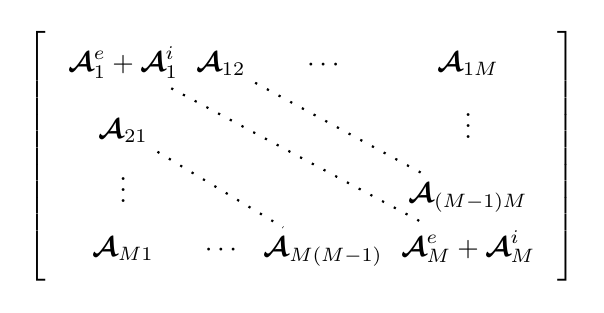
\begin{tikzpicture}[baseline={([yshift=-.5ex]current bounding box.center)}, ampersand replacement=\&]
\matrix (m) [matrix of math nodes,nodes in empty cells,right delimiter={]},left delimiter={[} ]{
\bm{\mathcal{{A}}}^e_1+\bm{\mathcal{{A}}}^i_1  \& \bm{\mathcal{{A}}}_{12}   \& \cdots  \& \bm{\mathcal{{A}}}_{1M}  \\
\bm{\mathcal{{A}}}_{21}    \& \& \& \vdots \\
\vdots  \&   \& \& \bm{\mathcal{{A}}}_{(M-1)M}   \\
\bm{\mathcal{{A}}}_{M1}  \& \cdots  \& \bm{\mathcal{{A}}}_{M(M-1)}   \& \bm{\mathcal{{A}}}^e_M+\bm{\mathcal{{A}}}^i_M\\
} ;
\draw[loosely dotted,thick] (m-1-1)-- (m-4-4);
\draw[loosely dotted,thick] (m-1-2)-- (m-3-4);
\draw[loosely dotted,thick] (m-2-1)-- (m-4-3);
\end{tikzpicture},  
\bm{\mathcal{A}}^i = 
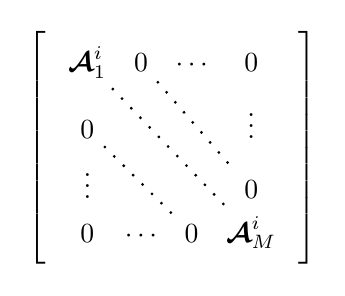
\begin{tikzpicture}[baseline={([yshift=-.5ex]current bounding box.center)}, ampersand replacement=\&]
\matrix (m) [matrix of math nodes,nodes in empty cells,right delimiter={]},left delimiter={[} ]{
\bm{\mathcal{{A}}}^i_1  \& 0   \& \cdots  \& 0  \\
0    \& \& \& \vdots \\
\vdots  \&   \& \& 0   \\
0 \& \cdots  \& 0 \& \bm{\mathcal{{A}}}^i_M\\
} ;
\draw[loosely dotted,thick] (m-1-1)-- (m-4-4);
\draw[loosely dotted,thick] (m-1-2)-- (m-3-4);
\draw[loosely dotted,thick] (m-2-1)-- (m-4-3);
\end{tikzpicture}, \nonumber\\
&\bm{\mathcal{I}} &=& 
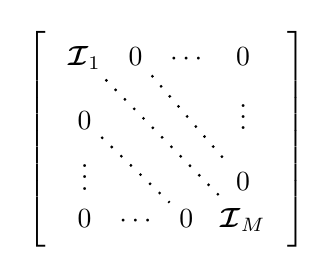
\begin{tikzpicture}[baseline={([yshift=-.5ex]current bounding box.center)}, ampersand replacement=\&]
\matrix (m) [matrix of math nodes,nodes in empty cells,right delimiter={]},left delimiter={[} ]{
\bm{\mathcal{{I}}}_1  \& 0   \& \cdots  \& 0  \\
0    \& \& \& \vdots \\
\vdots  \&   \& \& 0   \\
0 \& \cdots  \& 0 \& \bm{\mathcal{{I}}}_M\\
} ;
\draw[loosely dotted,thick] (m-1-1)-- (m-4-4);
\draw[loosely dotted,thick] (m-1-2)-- (m-3-4);
\draw[loosely dotted,thick] (m-2-1)-- (m-4-3);
\end{tikzpicture},  \quad 
\mathbf{u}^s = 
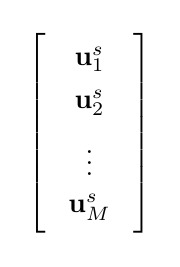
\begin{tikzpicture}[baseline={([yshift=-.5ex]current bounding box.center)}, ampersand replacement=\&]
\matrix (m) [matrix of math nodes,nodes in empty cells,right delimiter={]},left delimiter={[} ]{
{\mathbf{u}}^s_1    \\
{\mathbf{u}}^s_2  \\
\vdots   \\
{\mathbf{u}}^s_M\\
};
\end{tikzpicture},  \quad
\mathbf{u}^{inc} = 
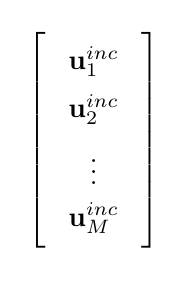
\begin{tikzpicture}[baseline={([yshift=-.5ex]current bounding box.center)}, ampersand replacement=\&]
\matrix (m) [matrix of math nodes,nodes in empty cells,right delimiter={]},left delimiter={[} ]{
{\mathbf{u}}^{inc}_1    \\
{\mathbf{u}}^{inc}_2  \\
\vdots   \\
{\mathbf{u}}^{inc}_M\\
}; \nonumber   
\end{tikzpicture}.
\end{align}
\end{scriptsize}
\end{frame}
%%%

%%%%
\begin{frame}{The PMCHWT formulation}
\begin{scriptsize}
\begin{align}
&\bm{\mathcal{A}} &=& 
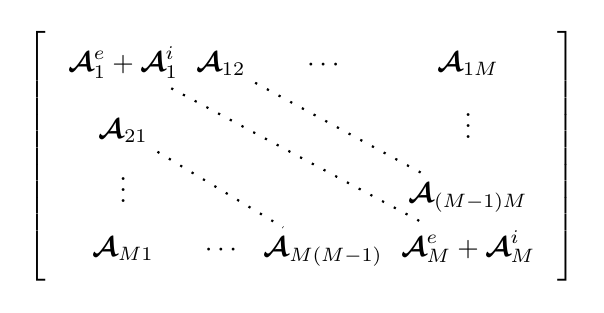
\begin{tikzpicture}[baseline={([yshift=-.5ex]current bounding box.center)}, ampersand replacement=\&]
\matrix (m) [matrix of math nodes,nodes in empty cells,right delimiter={]},left delimiter={[} ]{
\bm{\mathcal{{A}}}^e_1+\bm{\mathcal{{A}}}^i_1  \& \bm{\mathcal{{A}}}_{12}   \& \cdots  \& \bm{\mathcal{{A}}}_{1M}  \\
\bm{\mathcal{{A}}}_{21}    \& \& \& \vdots \\
\vdots  \&   \& \& \bm{\mathcal{{A}}}_{(M-1)M}   \\
\bm{\mathcal{{A}}}_{M1}  \& \cdots  \& \bm{\mathcal{{A}}}_{M(M-1)}   \& \bm{\mathcal{{A}}}^e_M+\bm{\mathcal{{A}}}^i_M\\
} ;
\draw[loosely dotted,thick] (m-1-1)-- (m-4-4);
\draw[loosely dotted,thick] (m-1-2)-- (m-3-4);
\draw[loosely dotted,thick] (m-2-1)-- (m-4-3);
\end{tikzpicture},   
\mathbf{u}^s = 
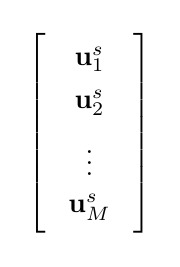
\begin{tikzpicture}[baseline={([yshift=-.5ex]current bounding box.center)}, ampersand replacement=\&]
\matrix (m) [matrix of math nodes,nodes in empty cells,right delimiter={]},left delimiter={[} ]{
{\mathbf{u}}^s_1    \\
{\mathbf{u}}^s_2  \\
\vdots   \\
{\mathbf{u}}^s_M\\
};
\end{tikzpicture},  \nonumber
\end{align}

    where
\begin{gather}
\bm{\mathcal{{A}}}^i_m = \begin{bmatrix}
\mathcal{C}^i_m & \frac{\mu_m}{k_m} \mathcal{S}^i_m \\[6pt]
-\frac{k_m}{\mu_m} \mathcal{S}^i_m & \mathcal{C}^i_m
\end{bmatrix}, \quad 
\bm{\mathcal{{A}}}^e_m = \begin{bmatrix}
\mathcal{C}^e_m & \frac{\mu_e}{k_e} \mathcal{S}^e_m \\[6pt]
-\frac{k_e}{\mu_e} \mathcal{S}^e_m & \mathcal{C}^e_m
\end{bmatrix}, \nonumber \\
\bm{\mathcal{{A}}}_{m\ell} = \begin{bmatrix}
    \mathcal{C}^e_{m\ell} & \frac{\mu_e}{k_e} \mathcal{S}^e_{m\ell} \\[6pt]
    -\frac{k_e}{\mu_e} \mathcal{S}^e_{m\ell} & \mathcal{C}^e_{m\ell}
\end{bmatrix}, \quad
%
{\mathbf{u}}^i_m = \begin{bmatrix}
    \gamma_{D,m}^{-} \mathbf{E}^i_m \\[6pt]
    \frac{k_m}{\mu_m} \gamma_{N,m}^- \mathbf{E}^i_m
\end{bmatrix}, \quad 
%
{\mathbf{u}}^s_m = \begin{bmatrix}
    \gamma_{D,m}^+ \mathbf{E}^s \\[6pt]
    \frac{k_e}{\mu_e} \gamma_{N,m}^+ \mathbf{E}^s
\end{bmatrix} \nonumber .
\end{gather}
\end{scriptsize}
\end{frame}
%%%%

%%%
\begin{frame}{Preconditioning: single scattering case}
    \begin{align}
        \bm{\mathcal{A}} = \bm{\mathcal{A}}_1^e + \bm{\mathcal{A}}_1^i = \begin{bmatrix}
            \mathcal{C}_1^e + \mathcal{C}_1^i & \frac{\mu_e}{k_e} \mathcal{S}_1^e + \frac{\mu_1}{k_1} \mathcal{S}_1^i \\
            -\frac{k_e}{\mu_e} \mathcal{S}^e_1 - \frac{k_1}{\mu_1} \mathcal{S}_1^i & \mathcal{C}_1^e + \mathcal{C}_1^i
        \end{bmatrix} \nonumber 
    \end{align}
    \pause 
    \begin{tikzpicture}
\hspace*{-0.6cm}
\node [anchor=west, bluecolour] (compact_top) at (-0.2,4) {\small Compact};
\node [anchor=west, bluecolour] (hypersingular_bottom) at (-0.8,1) {\small Hypersingular};

\node [anchor=west, bluecolour] (hypersingular_top) at (9,4) {\small Hypersingular};
\node [anchor=west, bluecolour] (compact_bottom) at (9,1) {\small Compact};
\begin{scope}[xshift=1.5cm]
    \node[anchor=south west,inner sep=0] (image) at (0,0) {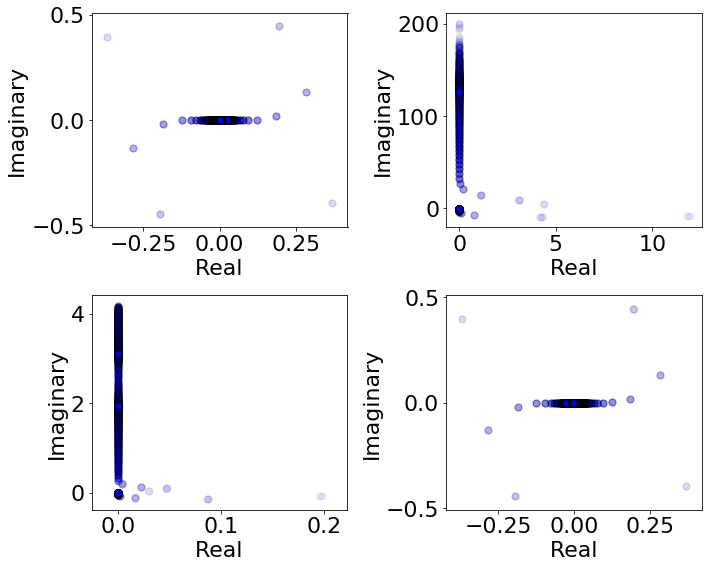
\includegraphics[width=0.7\textwidth]{Figures/eigenvalues_before.png}};
    \begin{scope}[x={(image.south east)},y={(image.north west)}]
        \draw [->, thick, bluecolour] (compact_top) to[out=90,in=180] (0.1,0.9);
        \draw [->, thick, bluecolour] (compact_bottom) to[out=270,in=0] (0.9,0.07);
        \draw [->, thick, bluecolour] (hypersingular_bottom) to[out=270,in=180] (0.1,0.07);
        \draw [->, thick, bluecolour] (hypersingular_top) to[out=90,in=0] (0.9,0.9);
    \end{scope}
\end{scope}
\end{tikzpicture}%
    % \begin{align}
    %     \only<1>{\bm{\mathcal{P}}\bm{\mathcal{A}}\mathbf{ u}^s = \bm{\mathcal{P}}\left(\frac{1}{2}\bm{\mathcal{ {I}}} - \bm{\mathcal{{A}}}^i \right) \mathbf{u}^{inc} \nonumber }
    %     \only<2>{\bm{\mathcal{A}}^2\mathbf{ u}^s = \bm{\mathcal{A}}\left(\frac{1}{2}\bm{\mathcal{ {I}}} - \bm{\mathcal{{A}}}^i \right) \mathbf{u}^{inc} \nonumber}
    % \end{align}
\end{frame}
%%%

%%%
\begin{frame}{Preconditioning: single scattering case}
\myfootnote{\fullcite{cools2011calderon}} 
    \begin{align}
        \bm{\mathcal{A}} = \bm{\mathcal{A}}_1^e + \bm{\mathcal{A}}_1^i = \begin{bmatrix}
            \mathcal{C}_1^e + \mathcal{C}_1^i & \frac{\mu_e}{k_e} \mathcal{S}_1^e + \frac{\mu_1}{k_1} \mathcal{S}_1^i \\
            -\frac{k_e}{\mu_e} \mathcal{S}^e_1 - \frac{k_1}{\mu_1} \mathcal{S}_1^i & \mathcal{C}_1^e + \mathcal{C}_1^i
        \end{bmatrix} \nonumber 
    \end{align}
    \pause 
    
    \begin{alignat}{2}
        \bm{\mathcal{P}}\bm{\mathcal{A}}\mathbf{ u}^s = \bm{\mathcal{P}}\left(\frac{1}{2}\bm{\mathcal{ {I}}} - \bm{\mathcal{{A}}}^i \right) \mathbf{u}^{inc} \nonumber  
    \end{alignat}
\end{frame}
%%%

%%%
\begin{frame}{Preconditioning: single scattering case}
\myfootnote{\fullcite{cools2011calderon}} 
    \begin{align}
        \bm{\mathcal{A}} = \bm{\mathcal{A}}_1^e + \bm{\mathcal{A}}_1^i = \begin{bmatrix}
            \mathcal{C}_1^e + \mathcal{C}_1^i & \frac{\mu_e}{k_e} \mathcal{S}_1^e + \frac{\mu_1}{k_1} \mathcal{S}_1^i \\
            -\frac{k_e}{\mu_e} \mathcal{S}^e_1 - \frac{k_1}{\mu_1} \mathcal{S}_1^i & \mathcal{C}_1^e + \mathcal{C}_1^i
        \end{bmatrix} \nonumber 
    \end{align}
    
    \begin{alignat}{2}
        \bm{\mathcal{A}}^2\mathbf{ u}^s = \bm{\mathcal{A}}\left(\frac{1}{2}\bm{\mathcal{ {I}}} - \bm{\mathcal{{A}}}^i \right) \mathbf{u}^{inc} \nonumber
    \end{alignat}
\end{frame}
%%%

%%%
\begin{frame}{Preconditioning: single scattering case}
\myfootnote{\fullcite{niino2012calderon}}
    \begin{tikzpicture}
\hspace*{-0.6cm}
\node [anchor=west, bluecolour] () at (-0.2,4) {$\alpha_1$, $\alpha_2$};
\node [anchor=west, bluecolour] (hypersingular_bottom) at (-0.8,1) {\small Compact};

\node [anchor=west, bluecolour] (hypersingular_top) at (9,4) {\small Compact};
\node [anchor=west, bluecolour] (compact_bottom) at (9,1) {$\alpha_1$, $\alpha_2$};
\begin{scope}[xshift=1.5cm]
    \node[anchor=south west,inner sep=0] (image) at (0,0) {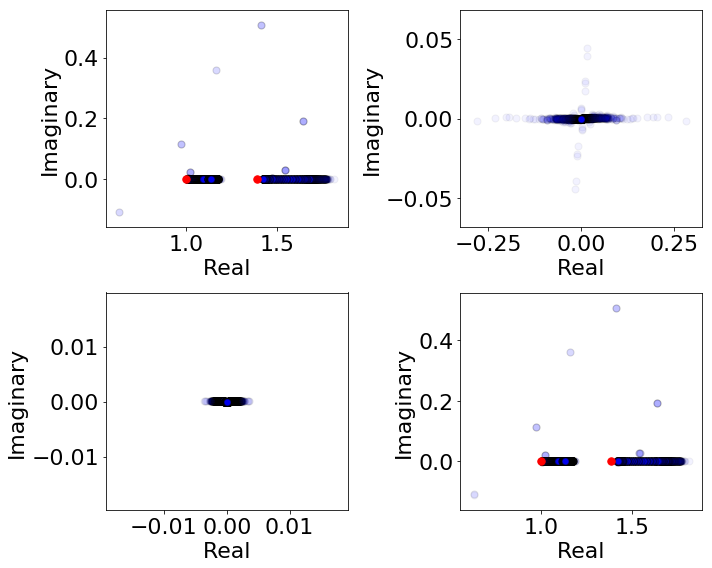
\includegraphics[width=0.7\textwidth]{Figures/eigenvalues_preconditioned.png}};
    \begin{scope}[x={(image.south east)},y={(image.north west)}]
        \draw [->, thick, bluecolour] (compact_top) to[out=90,in=180] (0.1,0.9);
        \draw [->, thick, bluecolour] (compact_bottom) to[out=270,in=0] (0.9,0.07);
        \draw [->, thick, bluecolour] (hypersingular_bottom) to[out=270,in=180] (0.1,0.07);
        \draw [->, thick, bluecolour] (hypersingular_top) to[out=90,in=0] (0.9,0.9);
    \end{scope}
\end{scope}
\end{tikzpicture}%
\vspace*{-1cm}
\begin{footnotesize}
\begin{eqnarray}
\alpha_1 = \frac{1}{2} + \frac{1}{4} \left( \frac{\mu_i}{\mu_e} + \frac{\mu_e}{\mu_i}\right), \quad
\alpha_2 = \frac{1}{2} + \frac{1}{4} \frac{\mu_i}{\mu_e} \left(\frac{k_e}{k_i}\right)^2 + \frac{1}{4} \frac{\mu_e}{\mu_i} \left( \frac{k_i}{k_e} \right)^2 \nonumber
\end{eqnarray}
\end{footnotesize}
\end{frame}
%%%

%%%
\begin{frame}{Preconditioning: multiple scattering case}
\begin{alignat}{3}
\bm{\mathcal{A}}\mathbf{ u}^s = \left(\frac{1}{2}\bm{\mathcal{ {I}}} - \bm{\mathcal{{A}}}^i \right) \mathbf{u}^{inc} \nonumber 
\end{alignat}
\pause
Full Calder\'on preconditioning:
\begin{align}
    \bm{\mathcal{A}}^2\mathbf{ u}^s = \bm{\mathcal{A}}\left(\frac{1}{2}\bm{\mathcal{ {I}}} - \bm{\mathcal{{A}}}^i \right) \mathbf{u}^{inc} \nonumber
\end{align}
\end{frame}
%%%

%%%
\begin{frame}{Preconditioning: multiple scattering case}
\begin{align}
&\bm{\mathcal{A}} &=& 
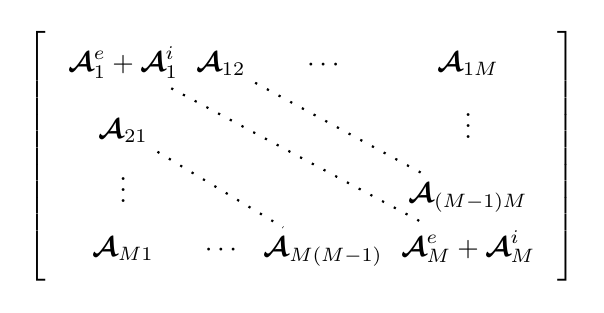
\begin{tikzpicture}[baseline={([yshift=-.5ex]current bounding box.center)}, ampersand replacement=\&]
\matrix (m) [matrix of math nodes,nodes in empty cells,right delimiter={]},left delimiter={[} ]{
\bm{\mathcal{{A}}}^e_1+\bm{\mathcal{{A}}}^i_1  \& \bm{\mathcal{{A}}}_{12}   \& \cdots  \& \bm{\mathcal{{A}}}_{1M}  \\
\bm{\mathcal{{A}}}_{21}    \& \& \& \vdots \\
\vdots  \&   \& \& \bm{\mathcal{{A}}}_{(M-1)M}   \\
\bm{\mathcal{{A}}}_{M1}  \& \cdots  \& \bm{\mathcal{{A}}}_{M(M-1)}   \& \bm{\mathcal{{A}}}^e_M+\bm{\mathcal{{A}}}^i_M\\
} ;
\draw[loosely dotted,thick] (m-1-1)-- (m-4-4);
\draw[loosely dotted,thick] (m-1-2)-- (m-3-4);
\draw[loosely dotted,thick] (m-2-1)-- (m-4-3);
\end{tikzpicture},   \nonumber
\end{align}
\end{frame}
%%%%

%%%
\begin{frame}{Preconditioning: multiple scattering case}
\begin{align}
&\bm{\mathcal{A}} &=& 
\begin{tikzpicture}[baseline={([yshift=-.5ex]current bounding box.center)}, ampersand replacement=\&]
\matrix (m) [matrix of math nodes,nodes in empty cells,right delimiter={]},left delimiter={[} ]{
\bm{\mathcal{{A}}}^e_1+\bm{\mathcal{{A}}}^i_1  \& \bm{\mathcal{{A}}}_{12}   \& \cdots  \& \bm{\mathcal{{A}}}_{1M}  \\
\bm{\mathcal{{A}}}_{21}    \& \& \& \vdots \\
\vdots  \&   \& \& \bm{\mathcal{{A}}}_{(M-1)M}   \\
\bm{\mathcal{{A}}}_{M1}  \& \cdots  \& \bm{\mathcal{{A}}}_{M(M-1)}   \& \bm{\mathcal{{A}}}^e_M+\bm{\mathcal{{A}}}^i_M\\
} ;
\draw[loosely dotted,thick] (m-1-1)-- (m-4-4);
\draw[loosely dotted,thick] (m-1-2)-- (m-3-4);
\draw[loosely dotted,thick] (m-2-1)-- (m-4-3);
\draw[bluecolour, opacity=.4,line width=6mm,line cap=round] (m-1-1.north west) -- (m-4-4.south east);
\end{tikzpicture},   \nonumber
\end{align}
\end{frame}
%%%%

%%%
\begin{frame}{Preconditioning: multiple scattering case}
\begin{alignat}{3}
\bm{\mathcal{A}}\mathbf{ u}^s = \left(\frac{1}{2}\bm{\mathcal{ {I}}} - \bm{\mathcal{{A}}}^i \right) \mathbf{u}^{inc} \nonumber 
\end{alignat}
Full Calder\'on preconditioning:
\begin{align}
    \bm{\mathcal{A}}^2\mathbf{ u}^s = \bm{\mathcal{A}}\left(\frac{1}{2}\bm{\mathcal{ {I}}} - \bm{\mathcal{{A}}}^i \right) \mathbf{u}^{inc} \nonumber
\end{align}
\pause 
Diagonal Calder\'on preconditioning:
\begin{align}
    \bm{\mathcal{D}}\bm{\mathcal{A}}\mathbf{ u}^s = \bm{\mathcal{D}}\left(\frac{1}{2}\bm{\mathcal{ {I}}} - \bm{\mathcal{{A}}}^i \right) \mathbf{u}^{inc} \nonumber 
\end{align}
\end{frame}
%%%

%%%
\begin{frame}{Variational Problem}
    In general form, the transmission formulation is of the form
    \begin{align}
        \nonumber \bm{\mathcal{A}} \mathbf{u} = \mathbf{f},
    \end{align}
    where
    \begin{itemize}
        \item $\bm{\mathcal{A}} :\mathbf{H}^{-\frac{1}{2}}_\times (\textnormal{div}_\Gamma, \Gamma)^2 \rightarrow \mathbf{H}^{-\frac{1}{2}}_\times (\textnormal{div}_\Gamma, \Gamma)^2$,
        \item $\mathbf{u} \in \mathbf{H}^{-\frac{1}{2}}_\times (\textnormal{div}_\Gamma, \Gamma)^2$,
        \item $\mathbf{f} \in \mathbf{H}^{-\frac{1}{2}}_\times (\textnormal{div}_\Gamma, \Gamma)^2$.
    \end{itemize}
    The dual of $\mathbf{H}^{-\frac{1}{2}}_\times (\textnormal{div}_\Gamma, \Gamma)^2$ with respect to the $L^2$ pairing is $\mathbf{H}^{-\frac{1}{2}}_\times (\textnormal{curl}_\Gamma, \Gamma)^2$.
    The transmission problem in variational form becomes
    \begin{align}
        \langle \bm{\mathcal{A}} \mathbf{u}, \mathbf{s}\rangle_{\mathbf{H}^{-\frac{1}{2}}_\times (\textnormal{div}_\Gamma, \Gamma) \times \mathbf{H}^{-\frac{1}{2}}_\times (\textnormal{curl}_\Gamma, \Gamma)} = \langle  \mathbf{f}, \mathbf{s}\rangle_{\mathbf{H}^{-\frac{1}{2}}_\times (\textnormal{div}_\Gamma, \Gamma) \times \mathbf{H}^{-\frac{1}{2}}_\times (\textnormal{curl}_\Gamma, \Gamma)}, \nonumber \\
        \forall \mathbf{s} \in  \nonumber \mathbf{H}^{-\frac{1}{2}}_\times (\textnormal{curl}_\Gamma, \Gamma)
    \end{align}
\end{frame}
%%%

%%%%
\begin{frame}{Galerkin discretisation}
    For the Galerkin method we need to choose discrete spaces
    \begin{itemize}
        \item $\mathbf{X}_h, \mathbf{Y}_h \in \mathbf{H}^{-\frac{1}{2}}_\times (\textnormal{div}_\Gamma, \Gamma)^2$, with basis functions $\{\mathbf{t}\}_{j=1}^J$, $\{\mathbf{p}\}_{j=1}^J$,
        \item $\mathbf{Z}_h \in  \mathbf{H}^{-\frac{1}{2}}_\times (\textnormal{curl}_\Gamma, \Gamma)^2$, with basis functions $\{ \mathbf{s}\}_{j=1}^J$.
    \end{itemize}
    Then approximate $\mathbf{u}$ by its discrete version as a combination of the basis functions
    \begin{align}
    \mathbf{u}_h = \sum_{j=1}^J U_j \mathbf{t}_j \nonumber 
\end{align}
The boundary integral formulation in the discrete variational form becomes
\begin{align}
    \langle \bm{\mathcal{A}} \mathbf{u}_h, \mathbf{s}_h\rangle_{\mathbf{Y}_h \times \mathbf{Z}_h} = \langle  \mathbf{f}, \mathbf{s}_h \rangle_{\mathbf{Y}_h \times \mathbf{Z}_h} , \quad \forall \mathbf{s}_h \in \mathbf{Z}_h, \nonumber
\end{align}
corresponding to a system of linear equations
\begin{eqnarray}
\mathbf{Ax} = \mathbf{b}, \nonumber 
\end{eqnarray}
\end{frame}
%%%

%%%
\begin{frame}{Discrete Systems: Weak and Strong Forms}
\myfootnote{\fullcite{betcke2017product}}
    \begin{itemize}
    \item The Galerkin discretisation of $\bm{\mathcal{A}}\mathbf{ u}^s = \left(\frac{1}{2}\bm{\mathcal{ {I}}} - \bm{\mathcal{{A}}}^i \right) \mathbf{u}^{inc} $ gives
    \begin{align}
        \mathbf{A} \mathbf{x} = \mathbf{b} \quad \only<4>{\textnormal{\color{bluecolour}   WEAK FORM}}\nonumber
    \end{align}
    $\mathbf{A}_{ij} = \langle \bm{\mathcal{A}} \mathbf{t}_j,\mathbf{s}_i\rangle _{\mathbf{Y}_h \times \mathbf{Z}_h}$
    
    $\mathbf{t}_j:$ trial functions, 
    $\mathbf{s}_i$: test functions 
    \pause
    \item $\mathbf{A}$ maps from the domain space to the dual space of the range space. If instead we want to map from the domain to the range we multiply by some $\mathbf{M}^{-1}$ with $\mathbf{M}_{ij} = \langle \mathbf{p}_i, \mathbf{s}_j \rangle _{\mathbf{Y}_h \times \mathbf{Z}_h}$
    \pause
    \item Mass matrix preconditioning
    \begin{align}
        \mathbf{M}^{-1} \mathbf{A} \mathbf{x} = \mathbf{M}^{-1} \mathbf{b} \quad  \only<4>{\textnormal{\color{bluecolour}   STRONG FORM}} \nonumber
    \end{align}
    \end{itemize}
\end{frame}
%%%

%%%
\begin{frame}{Discrete Systems: Weak and Strong Forms}
\hspace*{-2cm}
\begin{footnotesize}
\begin{table}
\centering
\begin{tabular}{lll}
\toprule
Continuous  & Discrete Weak Form  & Discrete Strong Form        \\
operator & & \\
\midrule
$\bm{\mathcal{A}}$ & $\mathbf{A}\mathbf{x} = \mathbf{b}$& $\mathbf{M}^{-1}\mathbf{A}\mathbf{x} = \mathbf{M}^{-1}\mathbf{b}$ \\[5pt]
%
$\bm{\mathcal{A}}^2$ & $\mathbf{A}\mathbf{M}^{-1}\mathbf{A}\mathbf{x} = \mathbf{A}\mathbf{M}^{-1}\mathbf{b}
$ & $\mathbf{M}^{-1}\mathbf{A}\mathbf{M}^{-1}\mathbf{A}\mathbf{x} = \mathbf{M}^{-1}\mathbf{A}\mathbf{M}^{-1}\mathbf{b}
$\\[5pt]
%
$\bm{\mathcal{D}}\bm{\mathcal{A}}$ & $\mathbf{D}\mathbf{M}^{-1}\mathbf{A}\mathbf{x} = \mathbf{D}\mathbf{M}^{-1}\mathbf{b}
$ & $\mathbf{M}^{-1}\mathbf{D}\mathbf{M}^{-1}\mathbf{A}\mathbf{x} = \mathbf{M}^{-1}\mathbf{D}\mathbf{M}^{-1}\mathbf{b}
$\\[5pt]
\bottomrule
\end{tabular}
\end{table}
\end{footnotesize}
\end{frame}
%%%

%%%
\begin{frame}{Discrete Spaces}
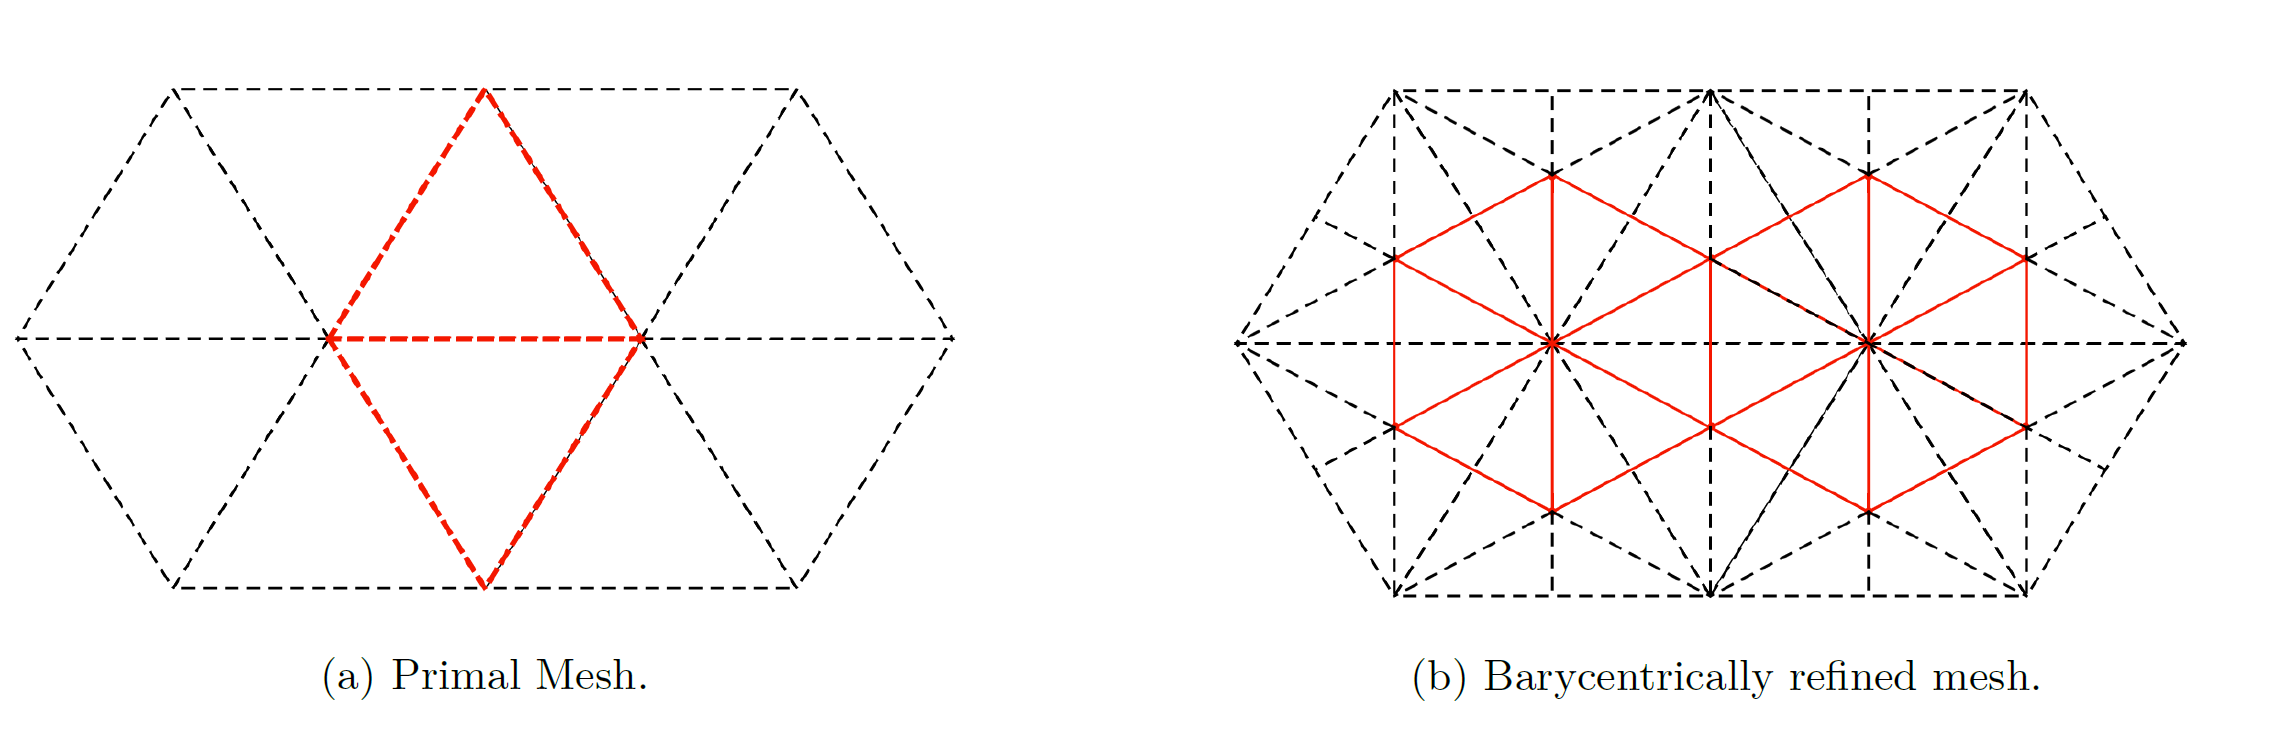
\includegraphics[width = 0.9 \textwidth]{Figures/basis_functions.png} 
\end{frame}
%%%

%%%
\begin{frame}{Discrete Spaces}
    \myfootnote{\fullcite{scroggs2017software}} 
    \myfootnote{\fullcite{buffa2007dual}}
    To be able to form $\mathbf{M}^{-1}$, the basis functions $\phi_j$, $\psi_j$ need to be inf-sup stable. One such choice:
    
    \begin{eqnarray}
\mathbf{A} = \begin{bmatrix}
\mathbf{C}_1 &  \frac{\mu}{k}\mathbf{S}_1 \\
-\frac{k}{\mu}\mathbf{S}_2 & \mathbf{C}_2
\end{bmatrix} \nonumber
\end{eqnarray}
 
\begin{eqnarray}
\mathbf{C}_1&:& \textnormal{(RWG, RWG, BC)}, \nonumber \\
\mathbf{S}_1&:& \textnormal{(BC, RWG, BC)}, \nonumber \\
\mathbf{C}_2&:& \textnormal{(BC, BC, RWG)}, \nonumber \\
\mathbf{S}_2&:& \textnormal{(RWG, BC, RWG)},  \nonumber
\end{eqnarray}
\end{frame}
%%%



%%%
\begin{frame}{Computational Complexity}
\begin{itemize}
\item matvec: a single application of one discretised boundary integral operator $\mathcal{C}^i_m$, $\mathcal{C}^e_m$, $\mathcal{S}^i_m$, $\mathcal{S}^e_m$. Applications of $\mathbf{M}^{-1}$ not taken into account
\end{itemize}

Total cost of operators:
    \begin{align}
        \bm{\mathcal{A}}&: 4M(M+1)(G + \floor*{ G/\rho}) \text{ matvecs} \nonumber \\
        \bm{\mathcal{A}}^2     &: 8M(M+1)(G + \floor*{ G/\rho}) + 4M(M+1)\text{ matvecs} \nonumber \\
        \bm{\mathcal{D}}\bm{\mathcal{A}}&: 4M(M +3) (G + \floor*{ G/\rho}) + 8M\text{ matvecs} \nonumber 
    \end{align}
$G$: number of GMRES iterations

$\rho$: number of iterations per GMRES cycle
\end{frame}
%%%

%%%
\begin{frame}{Benchmarks: single scattering}
\begin{footnotesize}
\begin{table}
\centering
\begin{tabular}{lrrrrr}
\toprule
& \multicolumn{2}{c}{$n=1.311 + 2.289 \times 10^{-9}\mathrm{i}$}  \\
\cmidrule{2-3}  
& $k_e=4$   & $k_e=10$       \\
\midrule
Discrete  &   &   \\
Operator & & \\
$\mathbf{A}$ & 599 (5024)  &  270 (2264) \\[4pt]
$\mathbf{M}^{-1} \mathbf{A}$ & 11 (88)  & 18 (144) \\[4pt]
$\mathbf{A}\mathbf{M}^{-1}\mathbf{A}$ &34 (568)    & 58 (968) \\[4pt]
$\mathbf{M}^{-1}\mathbf{A}\mathbf{M}^{-1}\mathbf{A}$ &6 (104)  &   10 (168) \\
\bottomrule
\end{tabular}
\end{table}
\end{footnotesize}
\end{frame}
%%%

%%%
\begin{frame}{Benchmarks: single scattering}
    \begin{figure}
    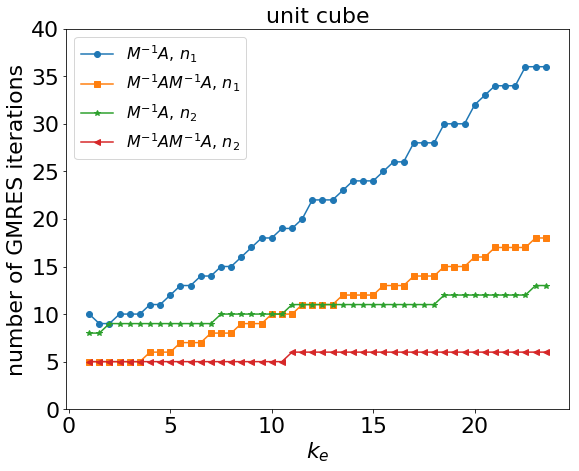
\includegraphics[width = 0.49\textwidth]{Figures/iterations.png}
    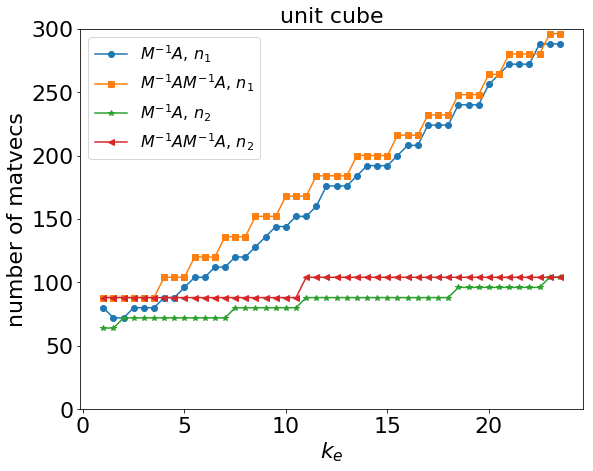
\includegraphics[width = 0.49\textwidth]{Figures/matvecs.png}
\end{figure}
$n_1=1.311 + 2.289 \times 10^{-9}\mathrm{i}$, \quad $n_2=1.0833 + 0.204 \mathrm{i}$
\end{frame}
%%%

%%%
\begin{frame}{Benchmarks: multiple scattering ($M=4$)}
% \vspace*{-1cm}
\begin{footnotesize}
\begin{table}
\centering
\begin{tabular}{lrrrrrr}
\toprule
& \multicolumn{2}{c}{$n=1.311 + 2.289 \times 10^{-9}i$}  \\
\cmidrule{2-3} 
 & $k_e =7$   & $k_e =22$ \\
\midrule
Discrete    &   &  & \\
operator & & & \\
$\mathbf{A}$  &326 (27360)  &406 (34080)  \\
$\mathbf{M}^{-1} \mathbf{A}$  &12 (960)  &24 (2000)\\
$\mathbf{A}\mathbf{M}^{-1} \mathbf{A}$   &32 (5360)   &122 (20560) \\
$\mathbf{M}^{-1} \mathbf{A}\mathbf{M}^{-1} \mathbf{A}$  &6 (1040)  &12 (2000) \\
$\mathbf{D}\mathbf{M}^{-1} \mathbf{A}$   &35 (4064)   &69 (8096) \\
$\mathbf{M}^{-1} \mathbf{D}\mathbf{M}^{-1} \mathbf{A}$  &7 (816)  &12 (1376)  \\
\bottomrule
\end{tabular}
\end{table}
\end{footnotesize}

\begin{figure}
    \hfill
    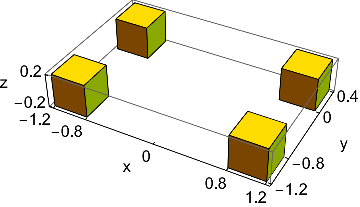
\includegraphics[width = 0.4 \textwidth]{Figures/4cubes.png}
\end{figure}
\end{frame}
%%%

%%%
\begin{frame}{\normalsize{Benchmarks: multiple scattering ($M=4, 8, 16$)}}
    \begin{figure}
    \centering
    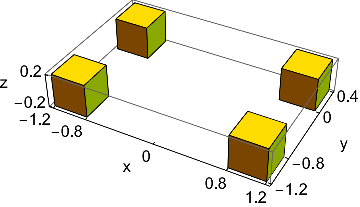
\includegraphics[width = 0.31 \textwidth]{Figures/4cubes.png}
    \hfill
    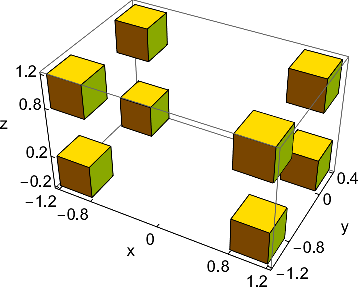
\includegraphics[width = 0.31 \textwidth]{Figures/8cubes.png}
    \hfill
    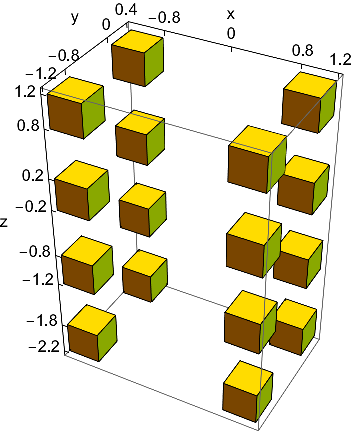
\includegraphics[width = 0.31 \textwidth]{Figures/16cubes.png}
\end{figure}

\begin{footnotesize}
\begin{table}
\centering
\begin{tabular}{lrrr}
\toprule
& \multicolumn{3}{c}{$n=1.311 + 2.289 \times 10^{-9}i$} \\
\cmidrule{2-4} 
& 4 cubes &  8 cubes & 16 cubes  \\
\midrule
Discrete operator   &   &  & \\
$\mathbf{M}^{-1} \mathbf{A}$ &22 (1840) &24 (7200) &32 (35904)  \\
$\mathbf{M}^{-1} \mathbf{A}\mathbf{M}^{-1} \mathbf{A}$ &11 (1840) &12 (7200) &16 (35904)   \\
$\mathbf{M}^{-1} \mathbf{D}\mathbf{M}^{-1} \mathbf{A}$ &12 (1376) &12 (4288) &16 (19584) \\
\bottomrule
\end{tabular}
\end{table}
\end{footnotesize}
\end{frame}
%%%

%%%
\begin{frame}{Benchmarks: multiple scattering ($M=4$)}
    \begin{figure}
\centering
    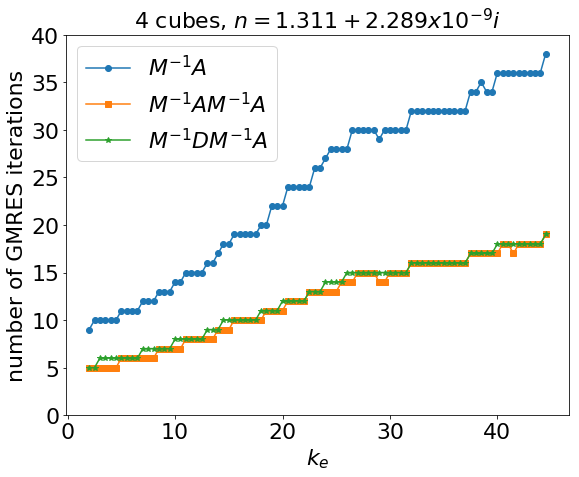
\includegraphics[width = 0.49 \textwidth]{Figures/iterations_multiple_low.png}
    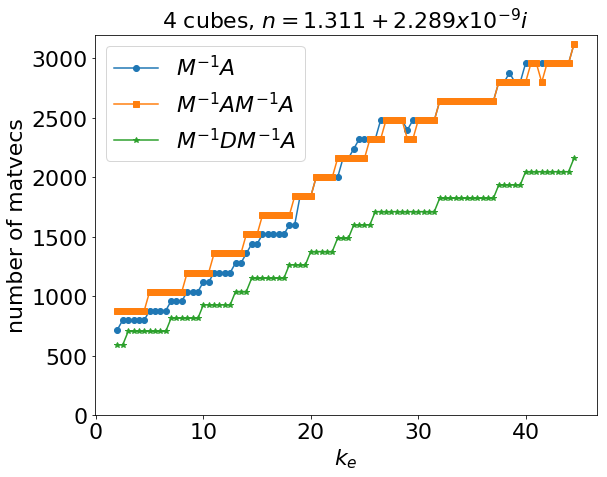
\includegraphics[width = 0.49 \textwidth]{Figures/matvecs_multiple_low.png}
\end{figure}
\end{frame}
%%%


% %%%
% \begin{frame}{Benchmarks: multiple scattering ($M=4$)}
%     \begin{figure}
% \centering
%     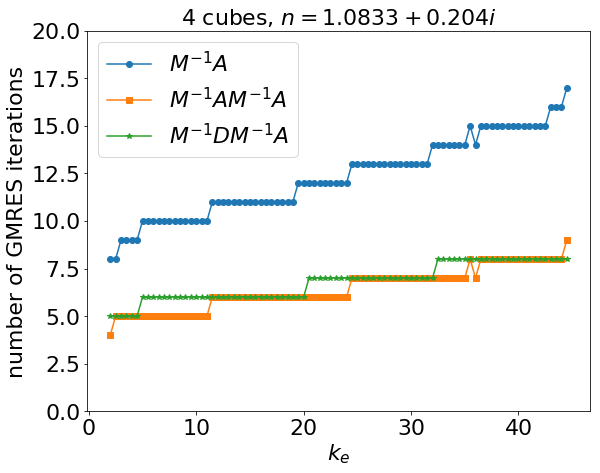
\includegraphics[width = 0.5 \textwidth]{Figures/iterations_multiple_high.png}
%     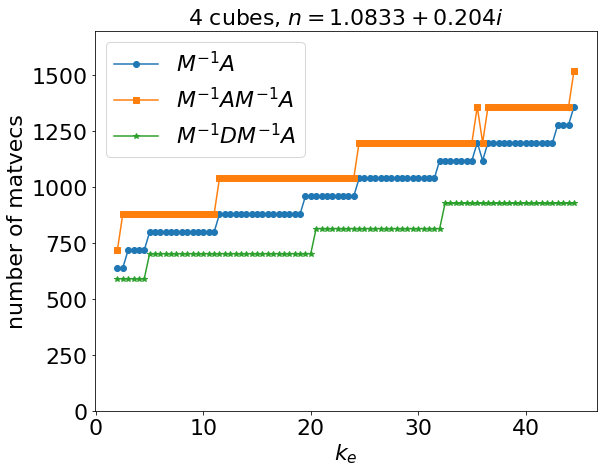
\includegraphics[width = 0.52 \textwidth]{Figures/matvecs_multiple_high.png}
% \end{figure}
% \end{frame}
% %%%

% %%%
% \begin{frame}{Benchmarks: distance of scatterers}
%     \begin{figure}
% 	\centering
%     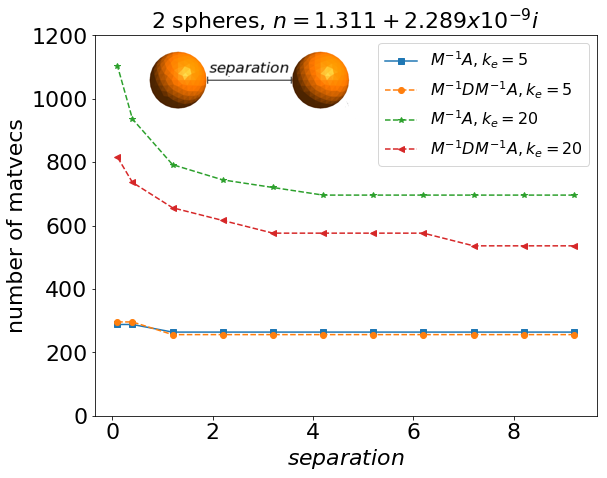
\includegraphics[width = 0.54\textwidth]{Figures/spheres_dist_low.png}
%     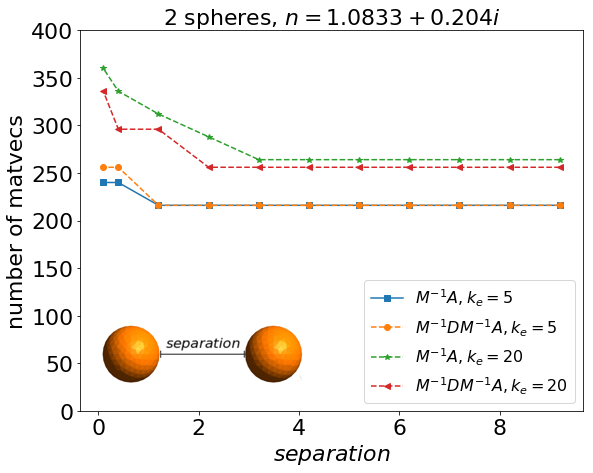
\includegraphics[width = 0.53 \textwidth]{Figures/spheres_dist_high.png}
%     \end{figure}
% \end{frame}
% %%%

%%%
\begin{frame}{Benchmarks: distance of scatterers}
    \begin{figure}
	\centering
    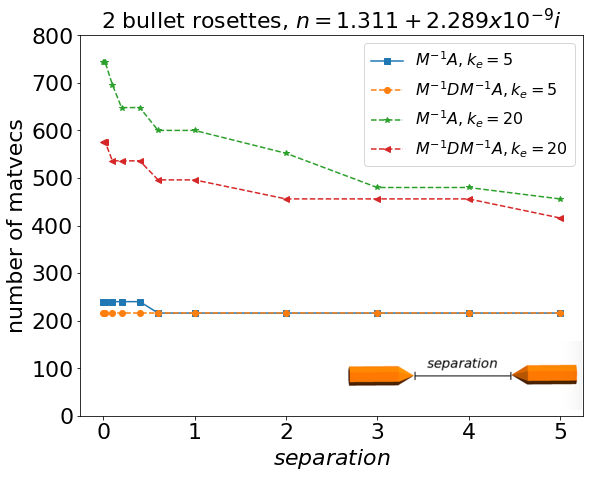
\includegraphics[width = 0.49\textwidth]{Figures/rosettes_dist_low.png}
    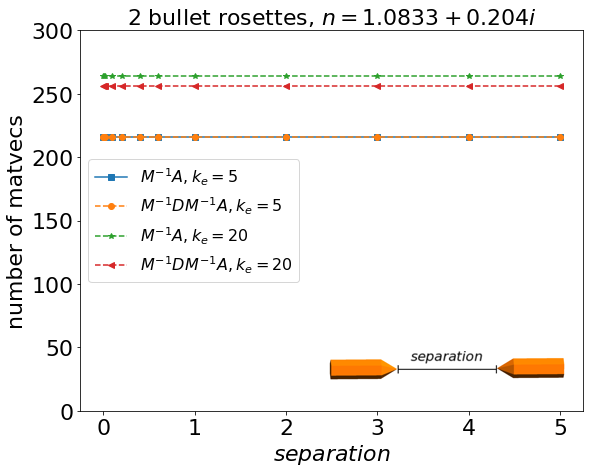
\includegraphics[width = 0.49 \textwidth]{Figures/rosettes_dist_high.png}
    \end{figure}
\end{frame}
%%%


%%%
\begin{frame}{Numerical Examples: single scattering}
    \begin{figure}
\centering
        \centering
        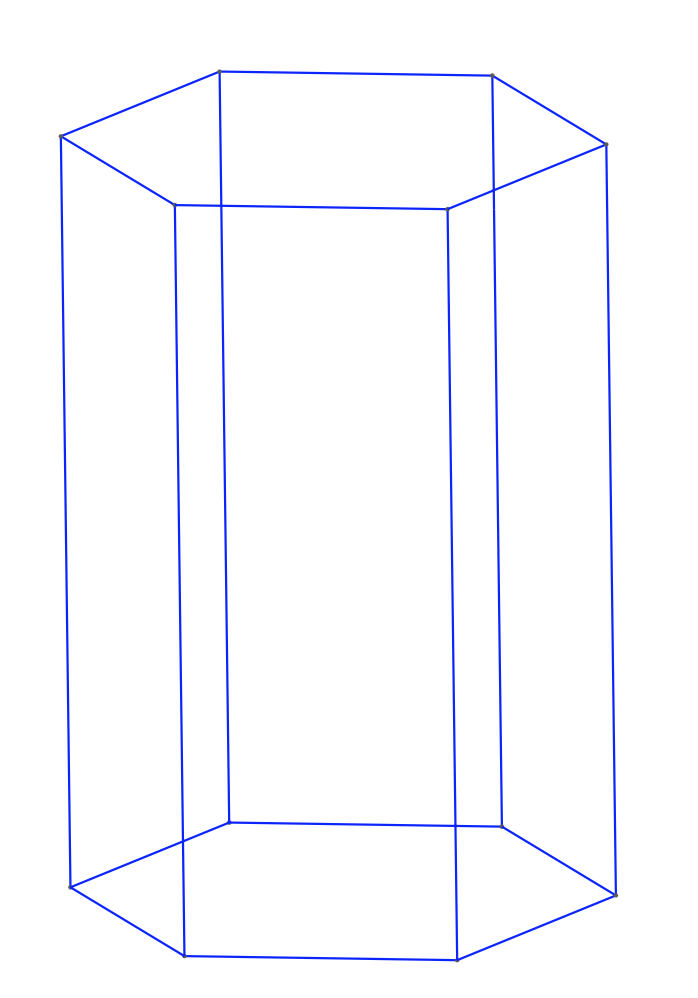
\includegraphics[height = 2cm]{Figures/hex.png} \hspace{2cm}%\hfill
        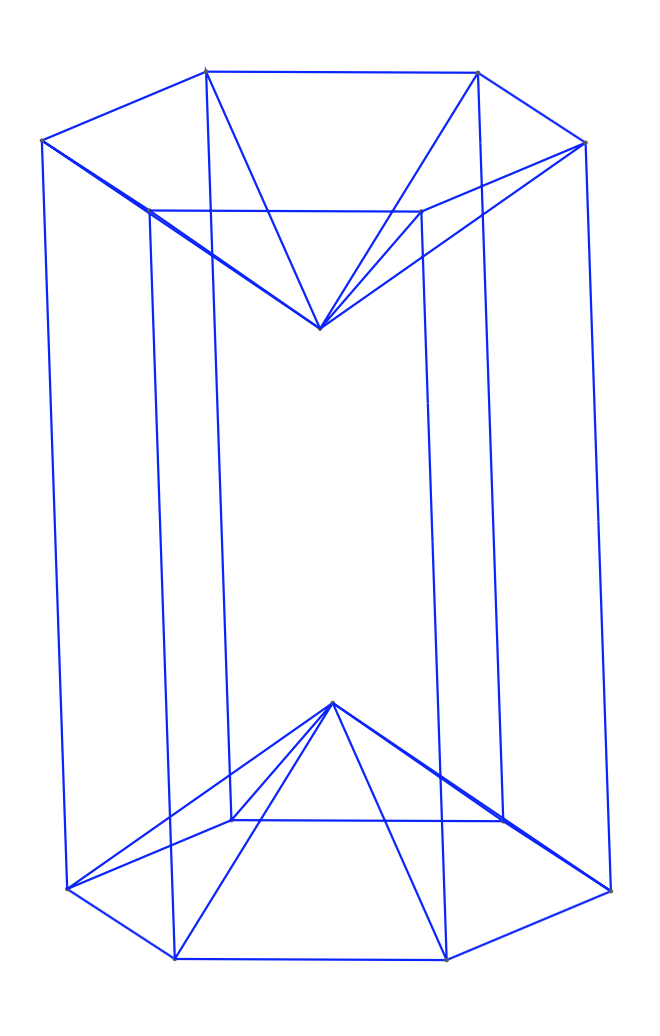
\includegraphics[height = 2.1cm]{Figures/cavity.png} \hspace{2cm}%\hfill
        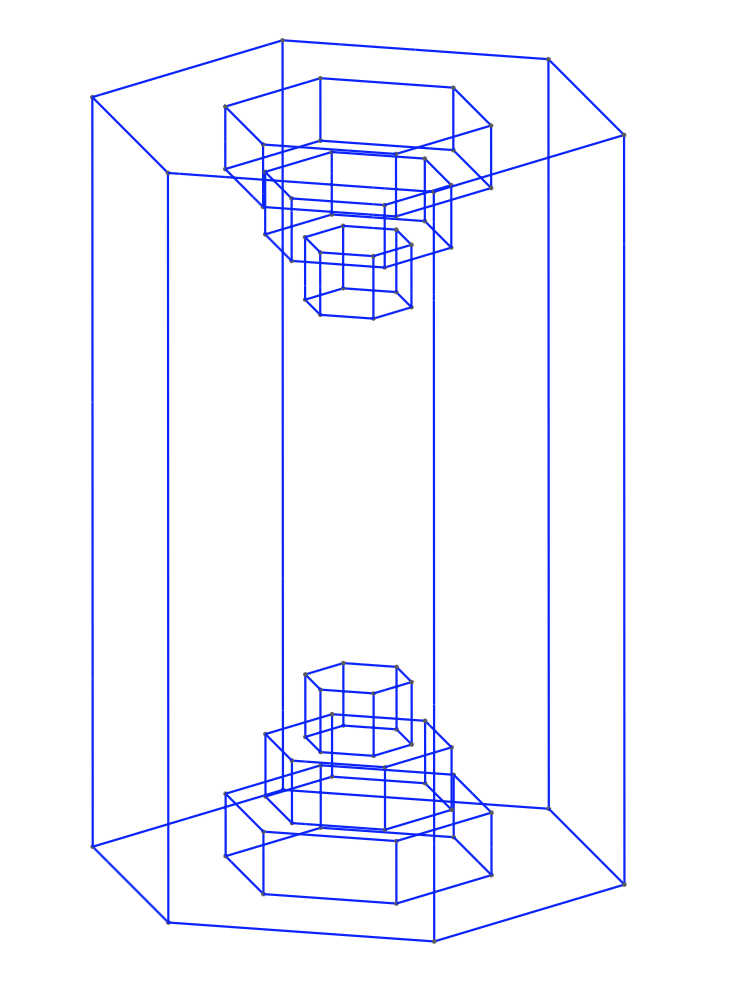
\includegraphics[height = 2cm]{Figures/cavity_stepped.png}
\end{figure}

\begin{figure}
        \centering
        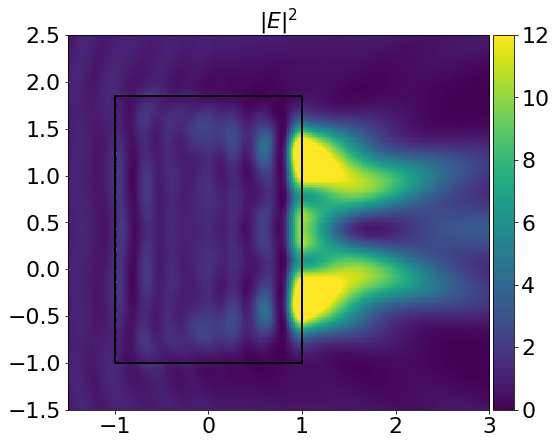
\includegraphics[width = 0.31 \textwidth]{Figures/hex_result.png} 
        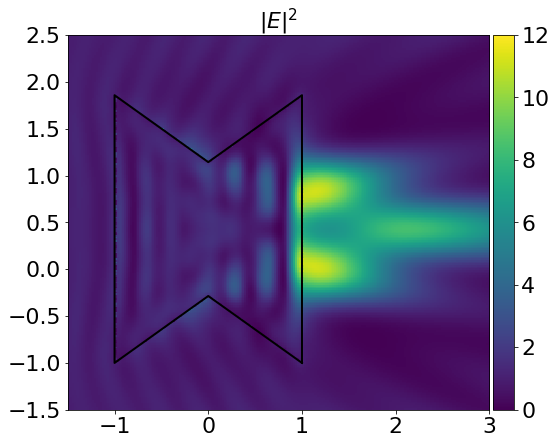
\includegraphics[width = 0.31 \textwidth]{Figures/cavity_result.png} 
        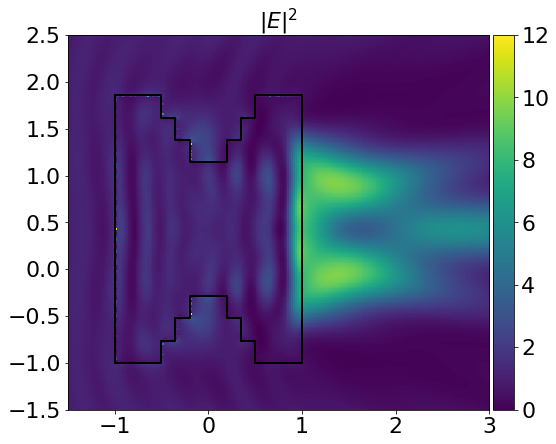
\includegraphics[width = 0.31 \textwidth]{Figures/stepped_cavity_result.png}
\end{figure}

\begin{footnotesize}
\begin{table}[t!]
\centering
\begin{tabular}{lrrr}
\toprule
& \multicolumn{3}{c}{$n=1.311 + 2.289 \times 10^{-9}\mathrm{i}$} \\
% \cmidrule{2-4} 
% & hexagonal &  with & with \\
% & column &  conventional & stepped \\
% &  &  cavity & cavity \\
\midrule
Discrete operator   &   &  & \\
$\mathbf{M}^{-1} \mathbf{A}$ & 34 (280) & 30 (248) & 34 (280)\\
$\mathbf{M}^{-1} \mathbf{A}\mathbf{M}^{-1} \mathbf{A}$ &17 (280) &15 (248) &17 (280)\\
\bottomrule
\end{tabular}
\end{table}
\end{footnotesize}
\end{frame}
%%%

%%%
\begin{frame}{Numerical Examples: multiple scattering}
    \begin{figure}
\centering
    \begin{subfigure}[t]{\textwidth}
        \centering
        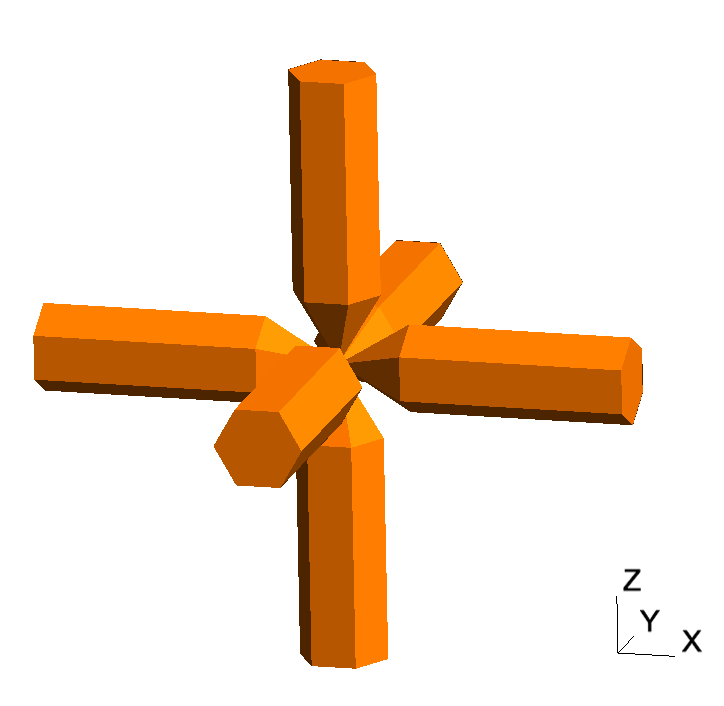
\includegraphics[height = 1.9cm]{Figures/6rosettes.png} \hspace{2cm}%\hfill
        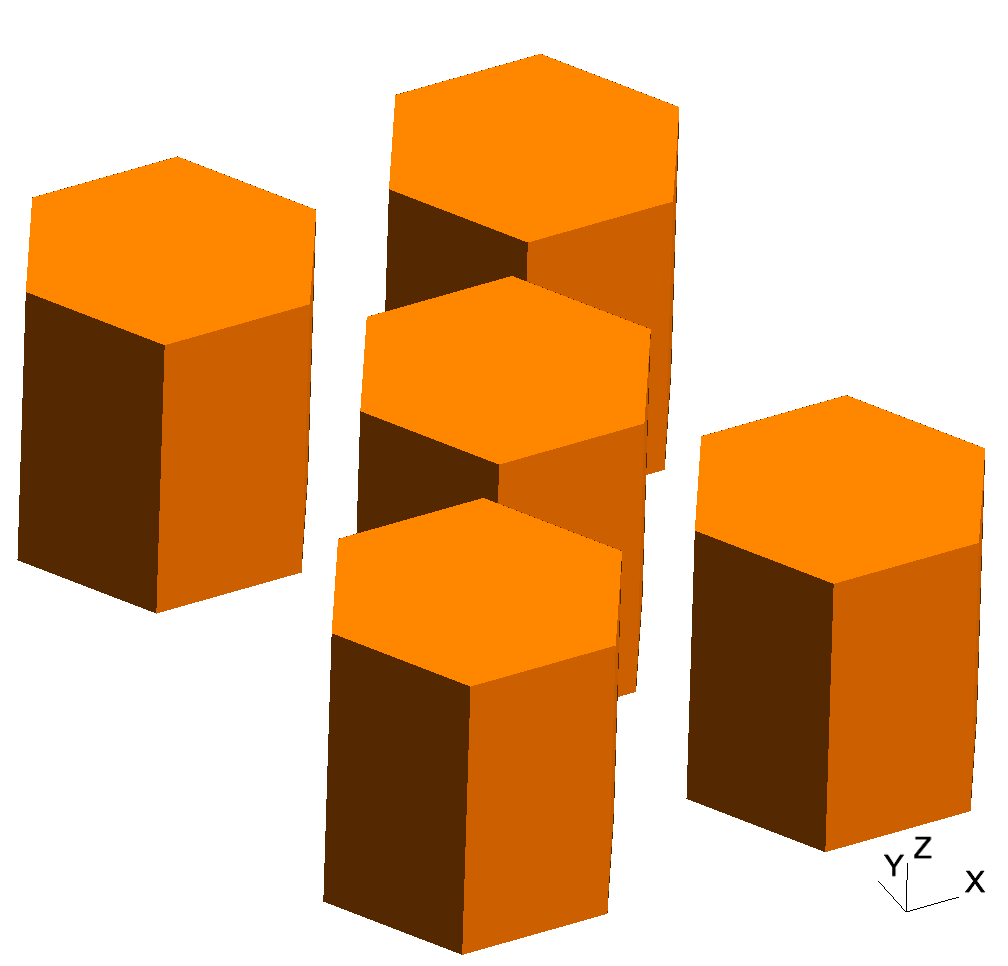
\includegraphics[height = 1.9cm]{Figures/5crystals.png} \hspace{3cm}%\hfill
        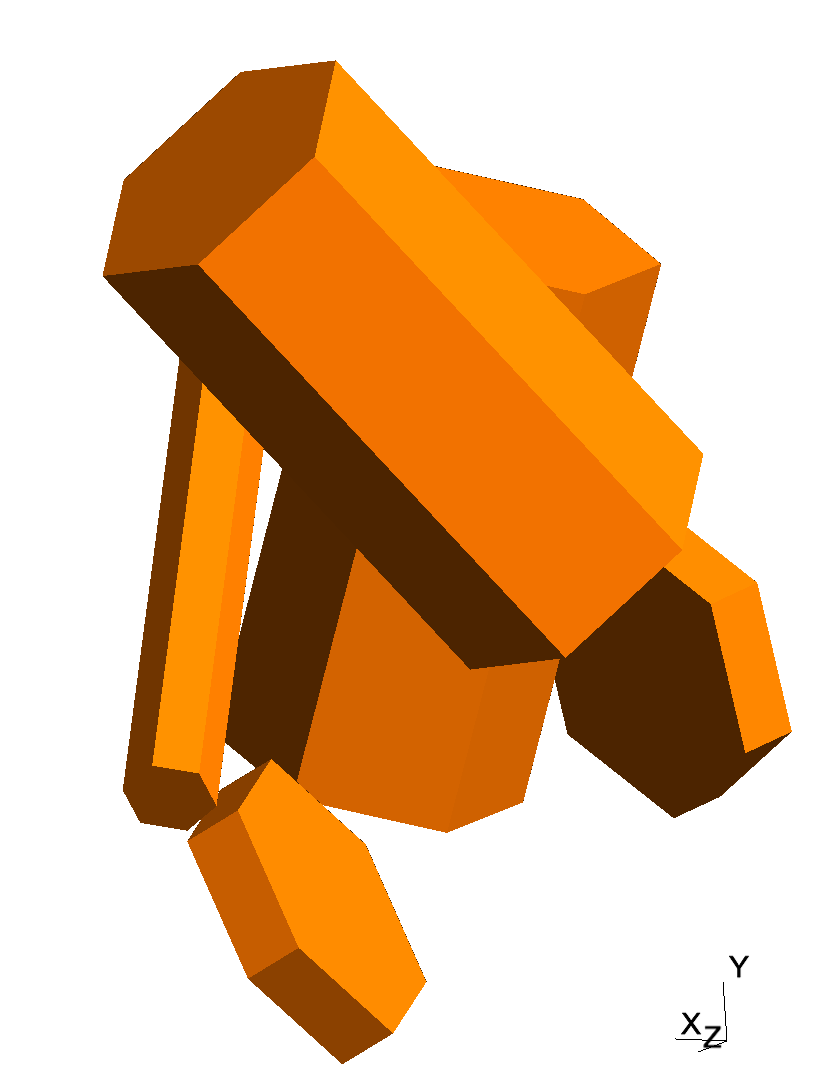
\includegraphics[height = 1.9cm]{Figures/5crystals_random.png}
    \end{subfigure}
    \begin{subfigure}[t]{\textwidth}
        \centering
        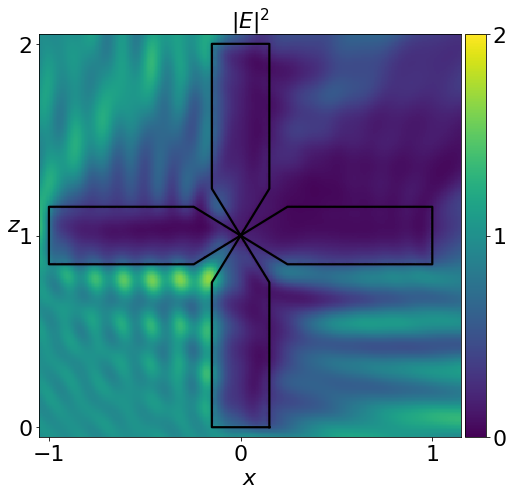
\includegraphics[width = 0.3 \textwidth]{Figures/6rosettes_result.png}
        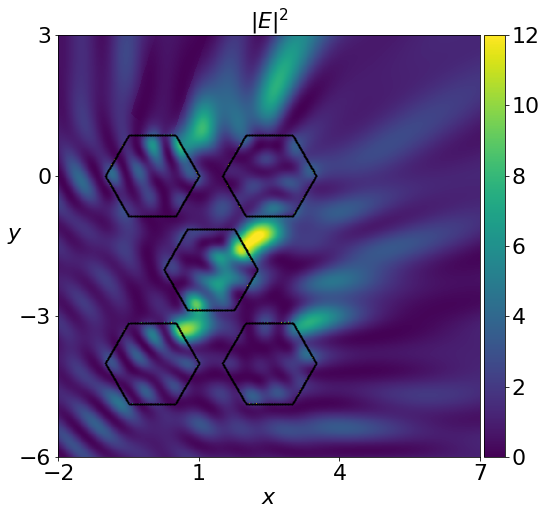
\includegraphics[width = 0.3 \textwidth]{Figures/5crystals_result.png}
        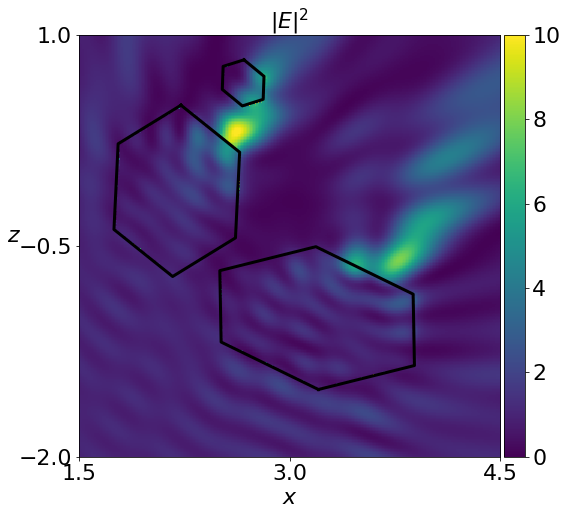
\includegraphics[width = 0.3 \textwidth]{Figures/5crystals_random_result.png}
    \end{subfigure}
\end{figure}

\begin{footnotesize}
\begin{table}
\centering
\begin{tabular}{lrrr}
% \toprule
% & 6-branch &  5 hex. & random \\
% & bullet &  columns & columns \\
% & rosette & & \\
\midrule
Discrete operator   &   &  & \\
$\mathbf{M}^{-1} \mathbf{A}$ & 15 (2520) & 52 (6480)  & 142 (17880)\\
$\mathbf{M}^{-1} \mathbf{A}\mathbf{M}^{-1} \mathbf{A}$ & 8 (2856) & 25 (6360) & 63 (15960)\\
$\mathbf{M}^{-1} \mathbf{D}\mathbf{M}^{-1} \mathbf{A}$ & 8 (1776) & 23 (3880) & 61 (10280)\\
\bottomrule
\end{tabular}
\end{table}
\end{footnotesize}
\end{frame}
%%%

%%%
\begin{frame}{Conclusion - part 1}
\myfootnote{\fullcite{kleanthous2019calderon}}
    % To summarise
    \begin{itemize}
        \item For single scattering: mass matrix preconditioning 
        \item For multiple scattering: strong form of block-diagonal Calder\'on preconditioning
    \end{itemize}
\end{frame}
%%%

\begin{frame}{Accelerated Calder\'on preconditioning}
\myfootnote{\fullcite{escapil2019fast}}
\begin{itemize}
    \item due to mesh refinement with exterior wavenumber $k_e$ simulations for large values are very slow and consume large amounts of memory
    \item how to minimise them?
    \item a bi-parametric implementation for EFIE problem has shown significant speedup in assembly time and lower memory requirements
\end{itemize}
\end{frame}

\begin{frame}{Accelerated Calder\'on preconditioning}
\myfootnote{\fullcite{escapil2019fast}}
The bi-parametric implementation:
\begin{itemize}
    \item split the accuracy of the operator and the preconditioner:
    \begin{itemize}
        \item high quadrature rules and small $\mathcal{H}$-matrix tolerance for the operator
        \item low quadrature rules and high $\mathcal{H}$-matrix tolerance for the preconditioner
    \end{itemize}
    \item use a different discretisation:
    \begin{itemize}
        \item use RWG functions for the operator
        \item use BC functions for the preconditioner
    \end{itemize}
\end{itemize}
In addition
\begin{itemize}
    \item include only near field interactions in the preconditioner
\end{itemize}
\end{frame}

\begin{frame}{Numerical Benchmarks}
\myfootnote{\fullcite{kleanthous2019accelerated}}
     \begin{figure}
	\centering
    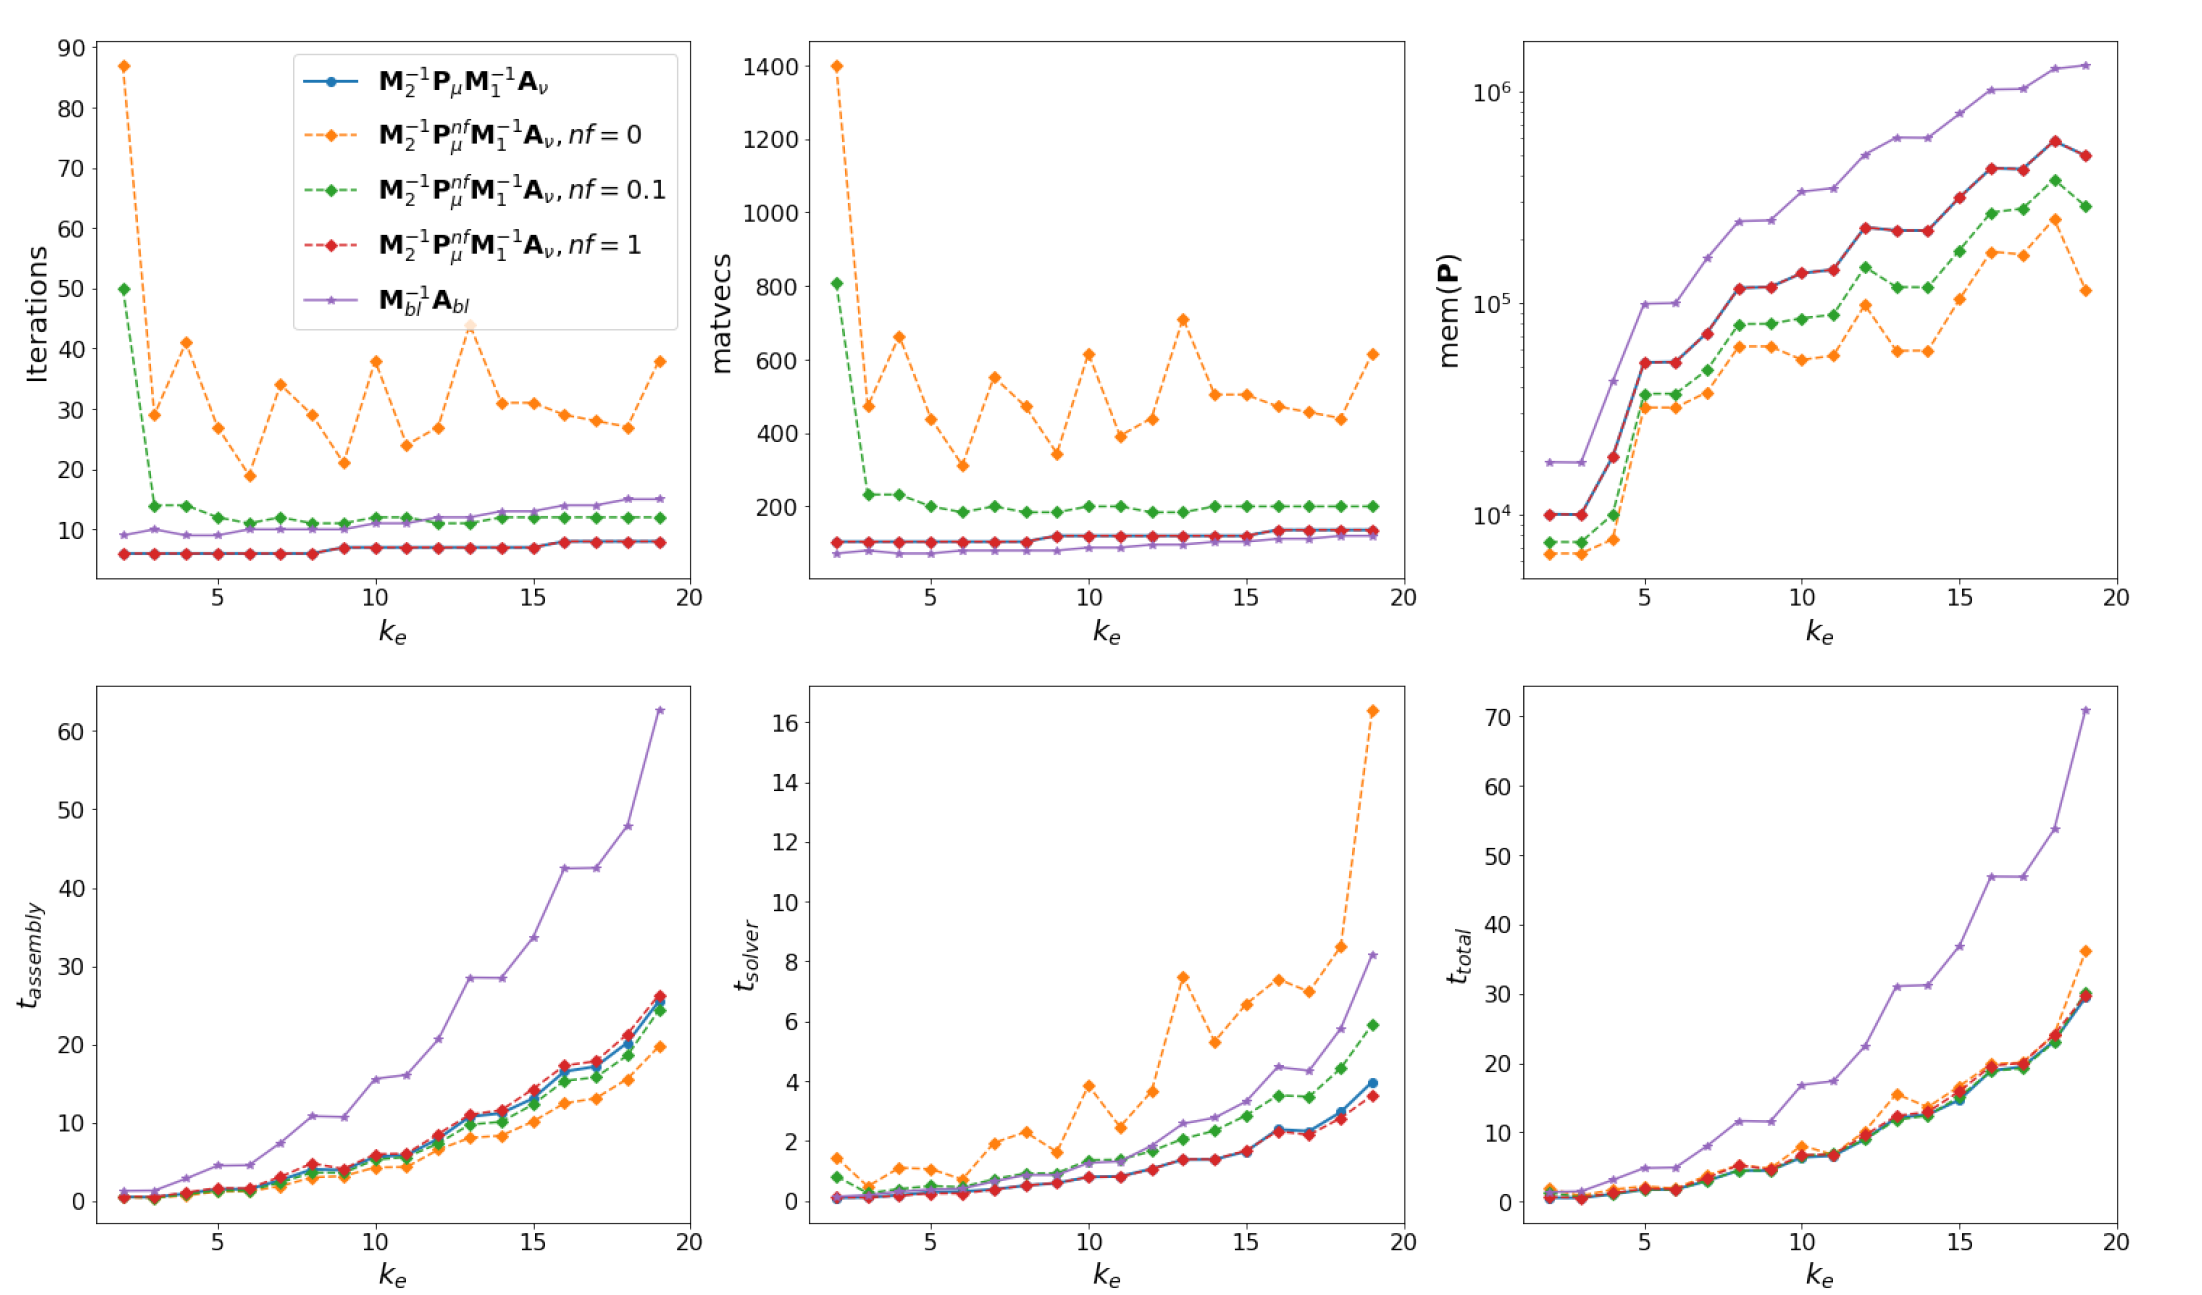
\includegraphics[width =  \textwidth]{Figures/multiple_low.png}
    \end{figure}
\end{frame}

\begin{frame}{Numerical Benchmarks: ice crystals}
    \begin{figure}
        \centering
        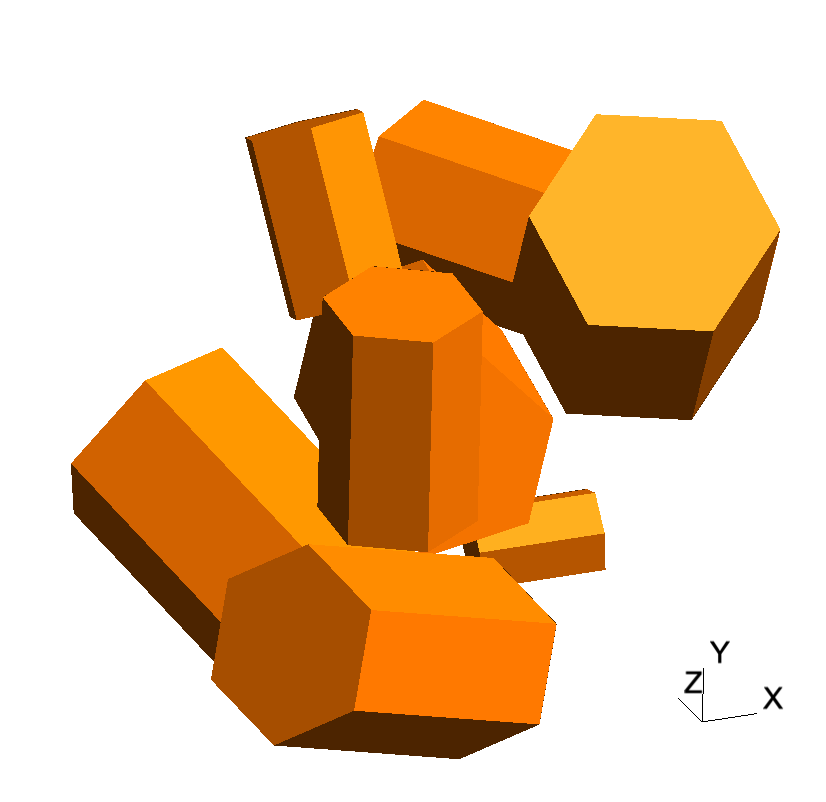
\includegraphics[width = 0.2 \textwidth]{Figures/8_agrr.png}
    \end{figure}
 
\vspace*{-1cm}

    \begin{figure}
        \centering
        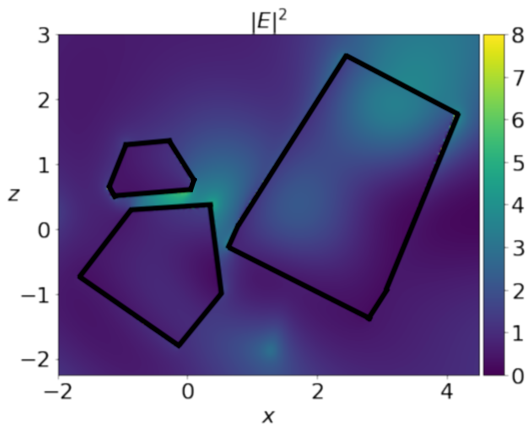
\includegraphics[width = 0.3 \textwidth]{Figures/50GHz_1cm.png} 
        \hfill
        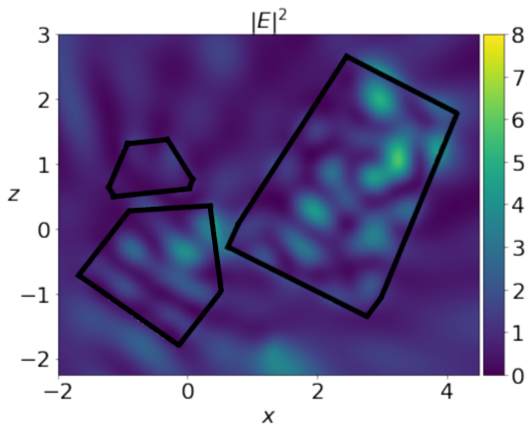
\includegraphics[width = 0.3 \textwidth]{Figures/183GHz_1cm.png}
        \hfill
        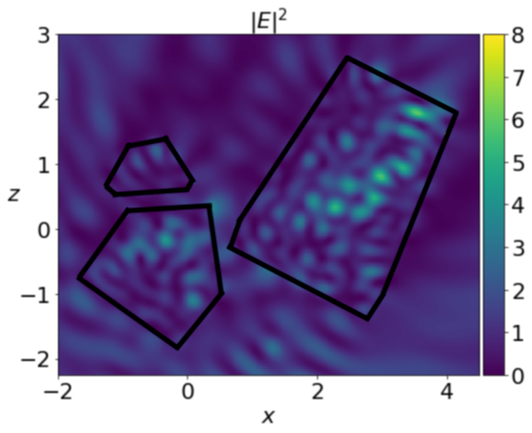
\includegraphics[width = 0.3 \textwidth]{Figures/325GHz_1cm.png}
    \end{figure}

\vspace*{-1cm}

    \begin{table}[ht!]
\centering
\resizebox{\textwidth}{!}{\begin{tabular}{llrrrrrrrrrr}
\toprule
$f$ & refractive index $n$ & elements & dofs & \multicolumn{2}{c}{Iterations} & \multicolumn{2}{c}{$t_{assembly}$ (mins)} & \multicolumn{2}{c}{$t_{solver}$ (mins)} & \multicolumn{2}{c}{$t_{total}$ (mins)} \\
\midrule
&&&& $\mathbf{DA}^{bl}_\nu$ &$\mathbf{ (DA)}^{nf}_{\mu,\nu}$ & $\mathbf{DA}^{bl}_\nu$ &$\mathbf{ (DA)}^{nf}_{\mu,\nu}$ & $\mathbf{DA}^{bl}_\nu$ &$\mathbf{ (DA)}^{nf}_{\mu,\nu}$ & $\mathbf{DA}^{bl}_\nu$ &$\mathbf{ (DA)}^{nf}_{\mu,\nu}$\\[5pt]
\midrule
$50$ & $1.7754+0.00066i$ & 2016 & 2556 & 46 & 37 & 3.4 & 0.45 & 0.9 & 0.21  & 4.3 &0.66 \\[5pt]
$183$ & $1.7754+0.00243i$ & 24896 & 26421 & 303 & 185 & 43.2 &6.15  &78.1 &10.58  & 121.3 &16.73 \\[5pt]
$325$ & $1.7754+0.0044i$ & 74208 & 81318 & - & 436 & - &21.9 & - & 97.2  & - & 119.1\\[5pt]
\bottomrule
\end{tabular}}
\end{table} 
\end{frame}

\begin{frame}{Conclusion - part 2}
\myfootnote{\fullcite{kleanthous2019accelerated}}
\begin{itemize}
    \item significant savings in assembly time and memory can be achieved with an accelerated implementation of Calder\'on preconditioning
    \item This includes
    
\begin{itemize}
    \item split the accuracy of the operator and the preconditioner:
    \begin{itemize}
        \item high quadrature rules and small $\mathcal{H}$-matrix tolerance for the operator
        \item low quadrature rules and high $\mathcal{H}$-matrix tolerance for the preconditioner
    \end{itemize}
    \item discretisation:
    \begin{itemize}
        \item use RWG functions for the operator
        \item use BC functions for the preconditioner
    \end{itemize}
    \item include only near field interactions in the preconditioner
\end{itemize}
\end{itemize}
    
\end{frame}

%%%
\begin{frame}{Work at the Met Office}
    \begin{itemize}
        \item Mid September - Mid December
        \item working with Anthony Baran
        \item goal is to simulate single scattering properties and phase matrices of aggregates of bullet rosettes in random orientation
        \item 5 temperatures: 190.0K, 210.0K, 230.0K, 250.0K, 270.0K
        \item 4 frequencies: 50GHz, 183GHz, 243GHz, 664GHz
        \item range of sizes ranging from $\mu m$ to $cm$.
    \end{itemize}
\end{frame}
%%%

%%%
\includepdf[page={-}]{Figures/MetOfficeInternship_presentation.pdf}
%%%

%%%
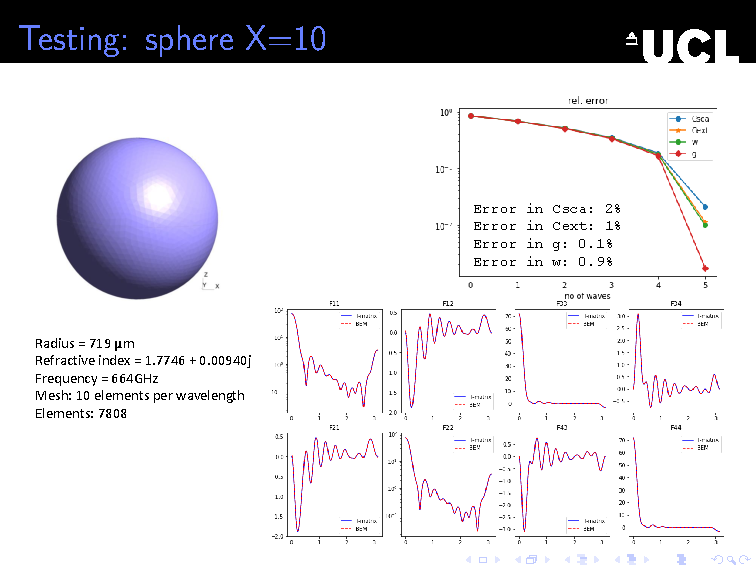
\includepdf[page = {-}]{Figures/MetOfficeInternship_presentation_testing.pdf}
%%%

%%%
\begin{frame}{Some results}
    \begin{figure}
        \centering
        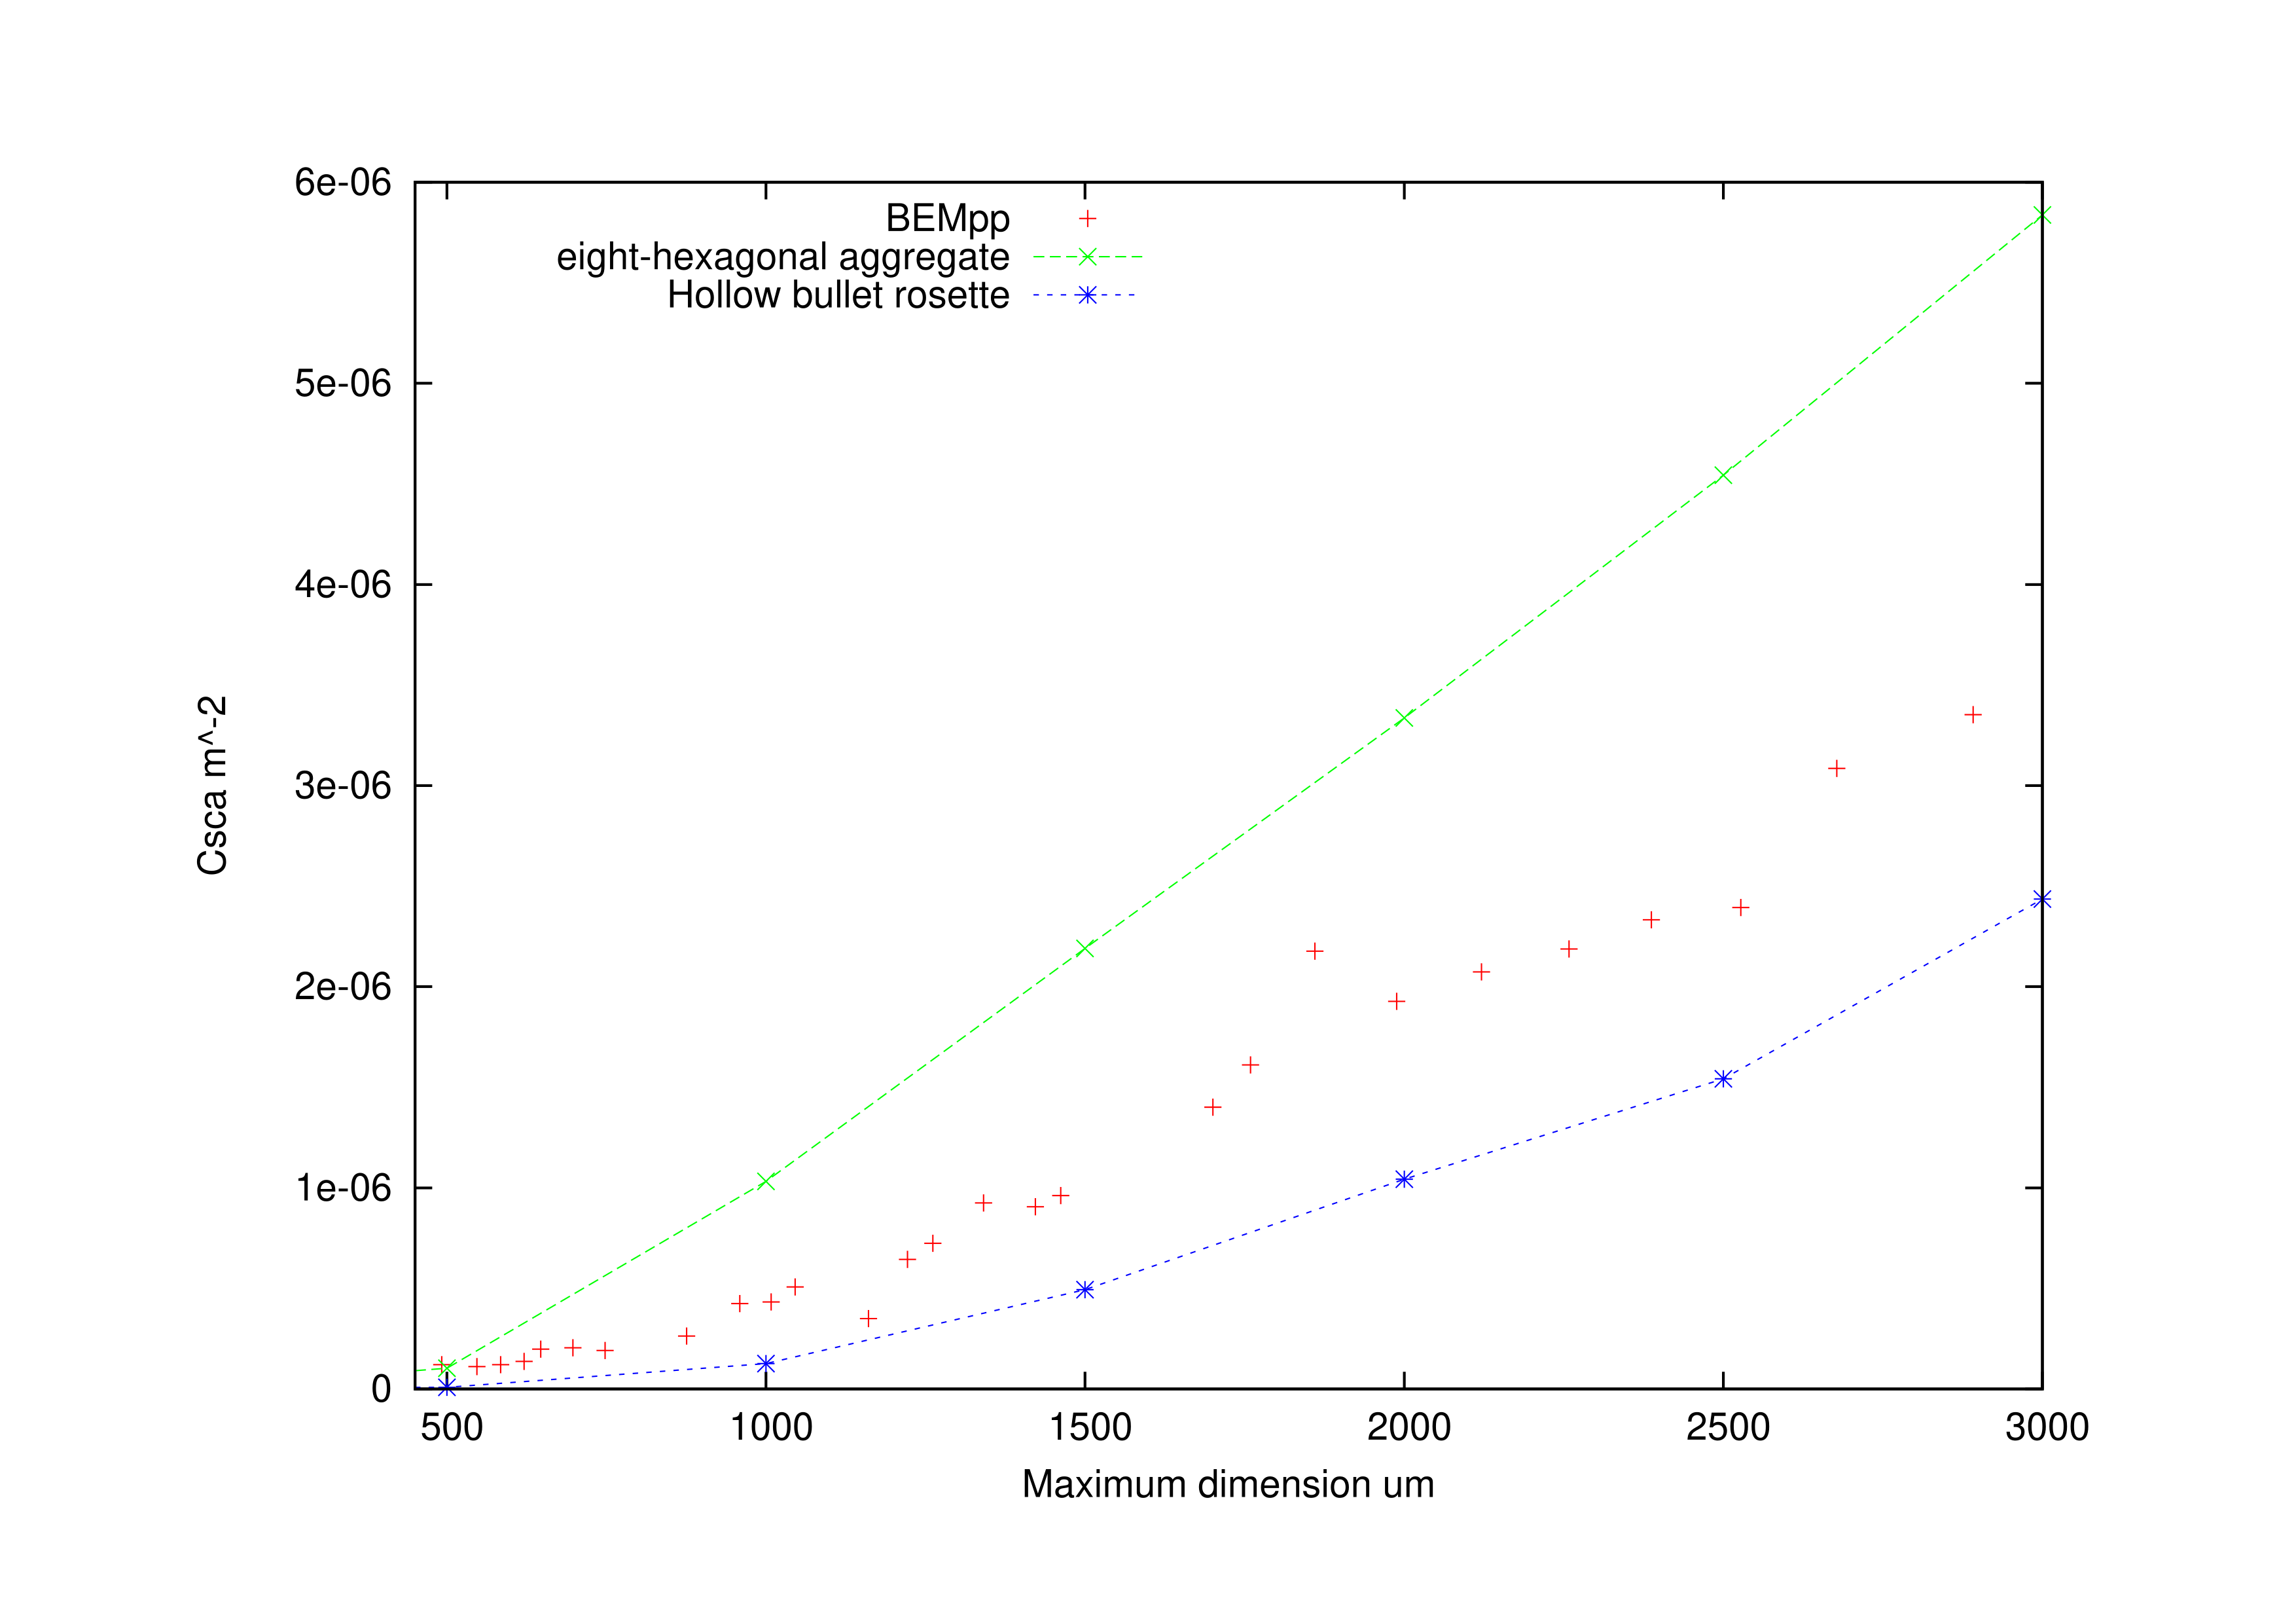
\includegraphics[width = 0.49 \textwidth]{Figures/rosette_aggregate_664ghz_tc_190_yang_csca.png}
        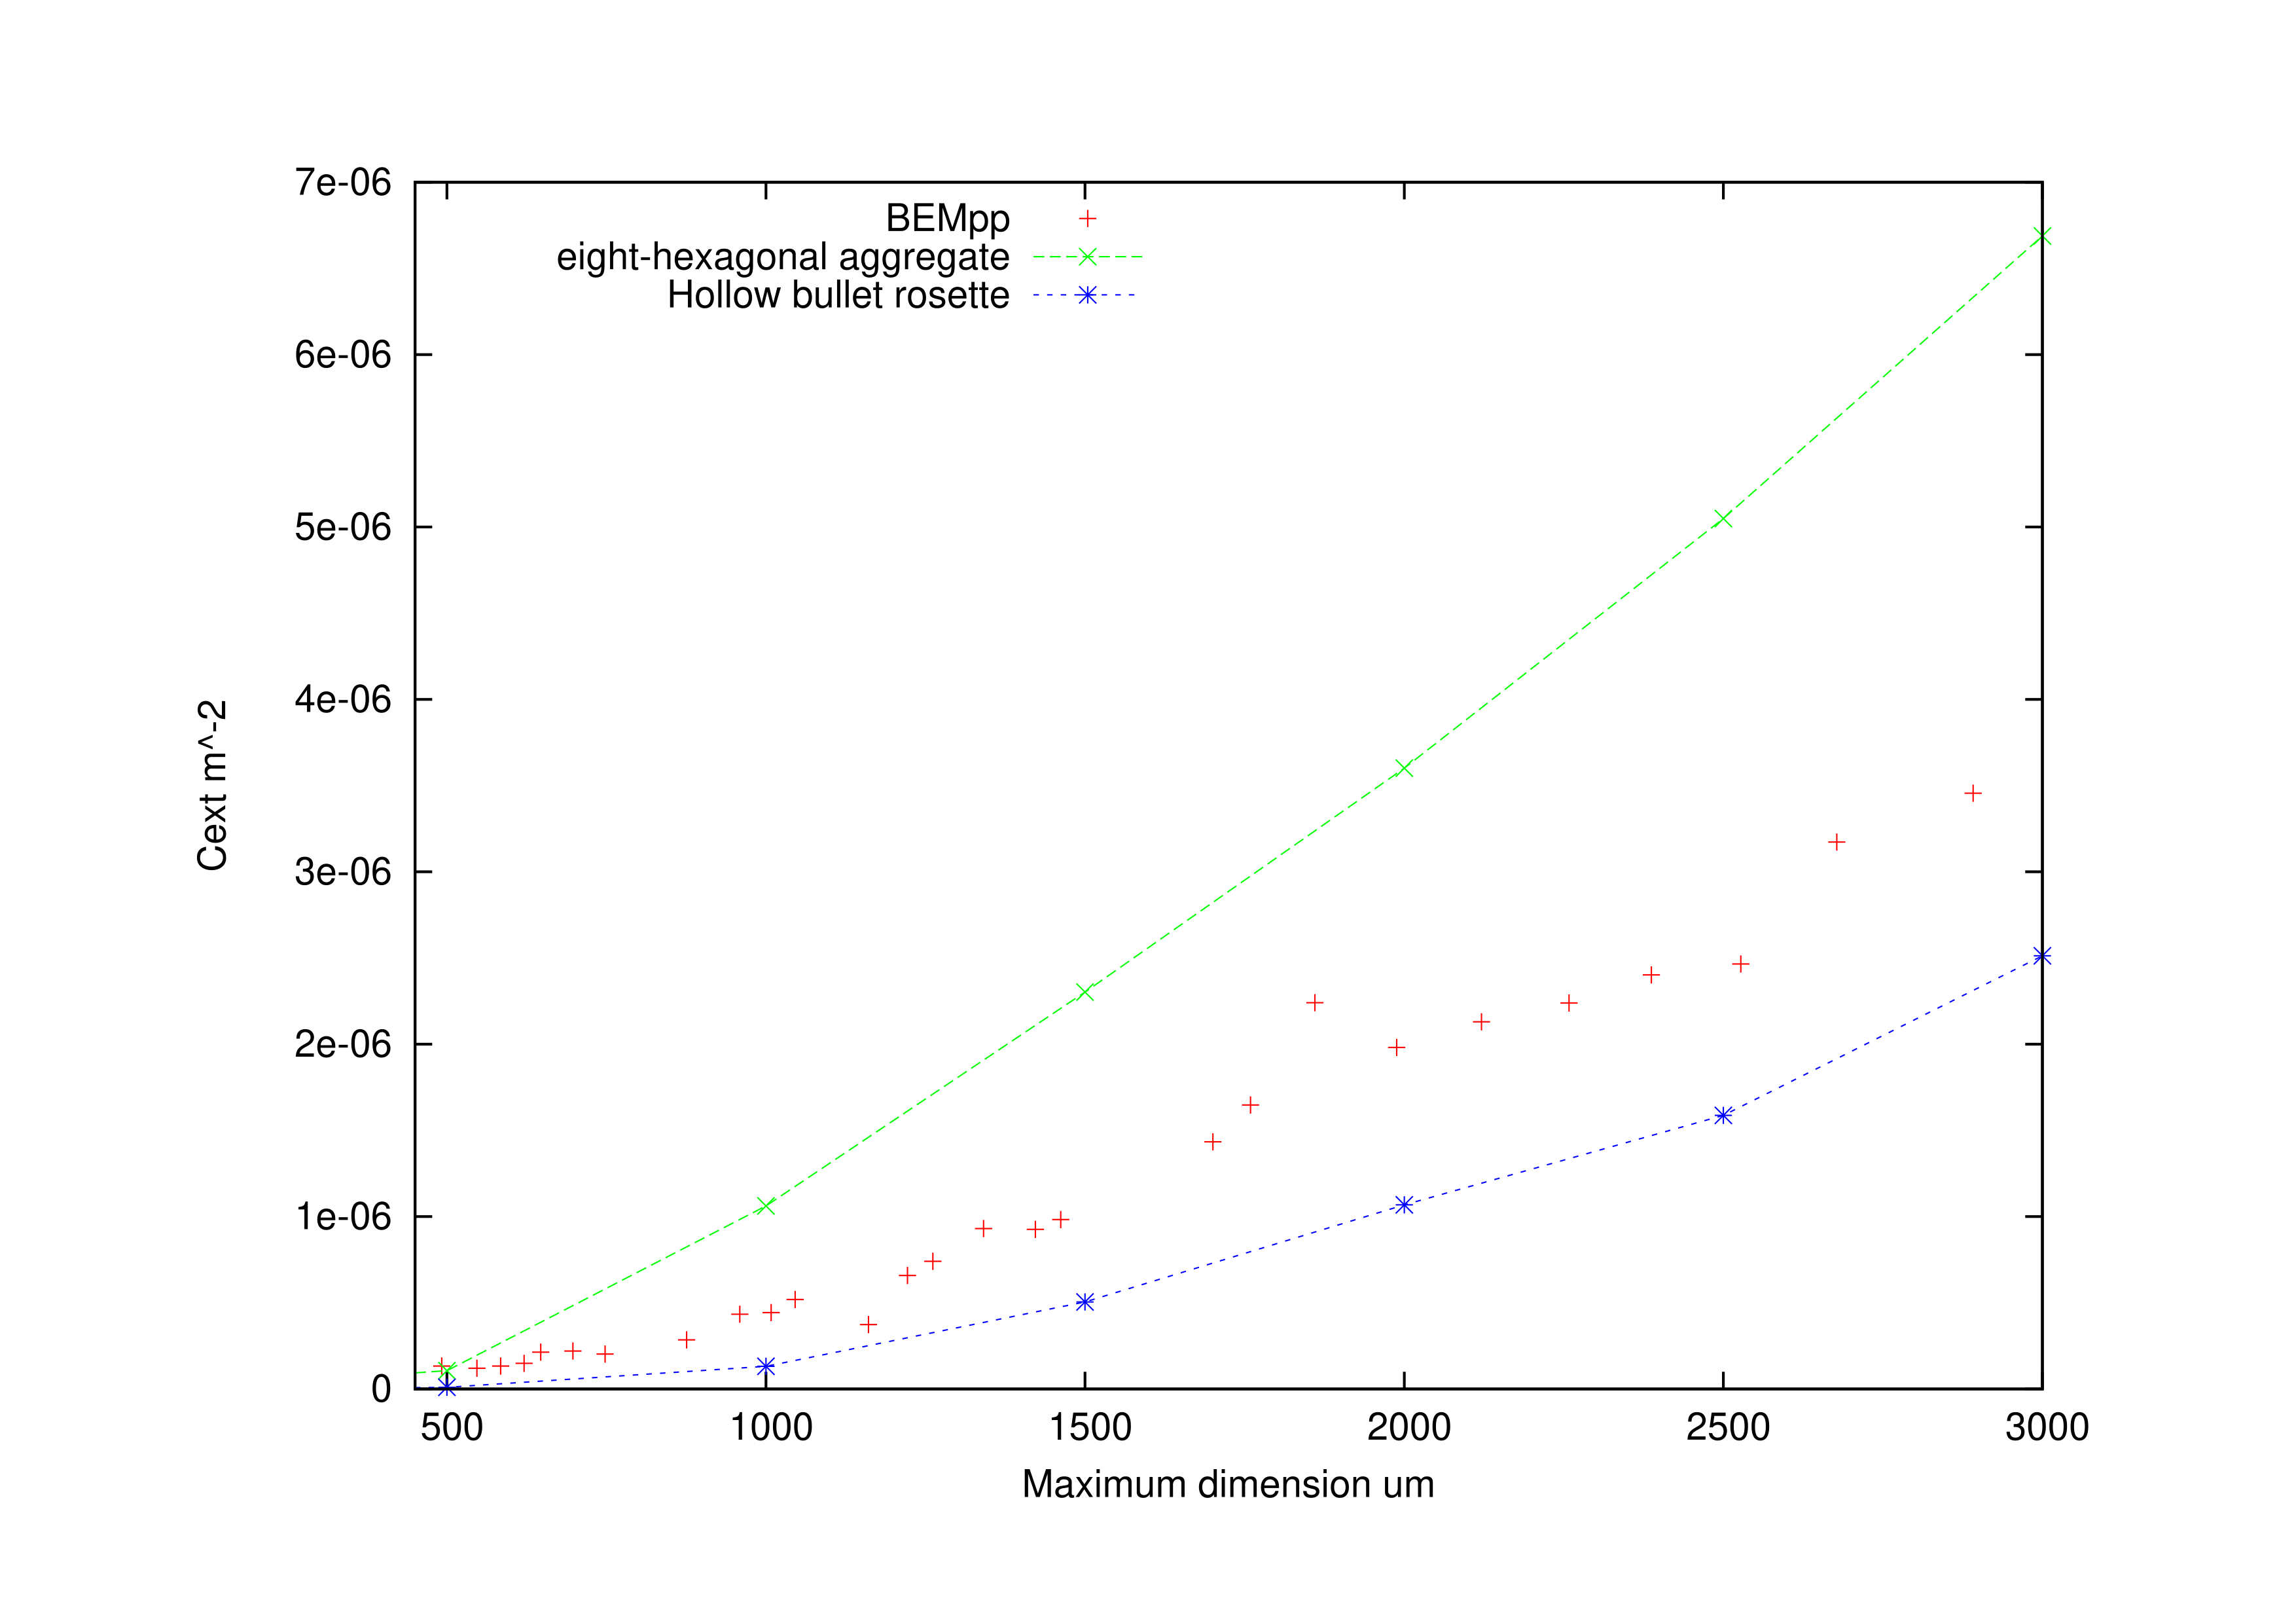
\includegraphics[width = 0.49 \textwidth]{Figures/rosette_aggregate_664ghz_tc_190_yang.png}
        \\
        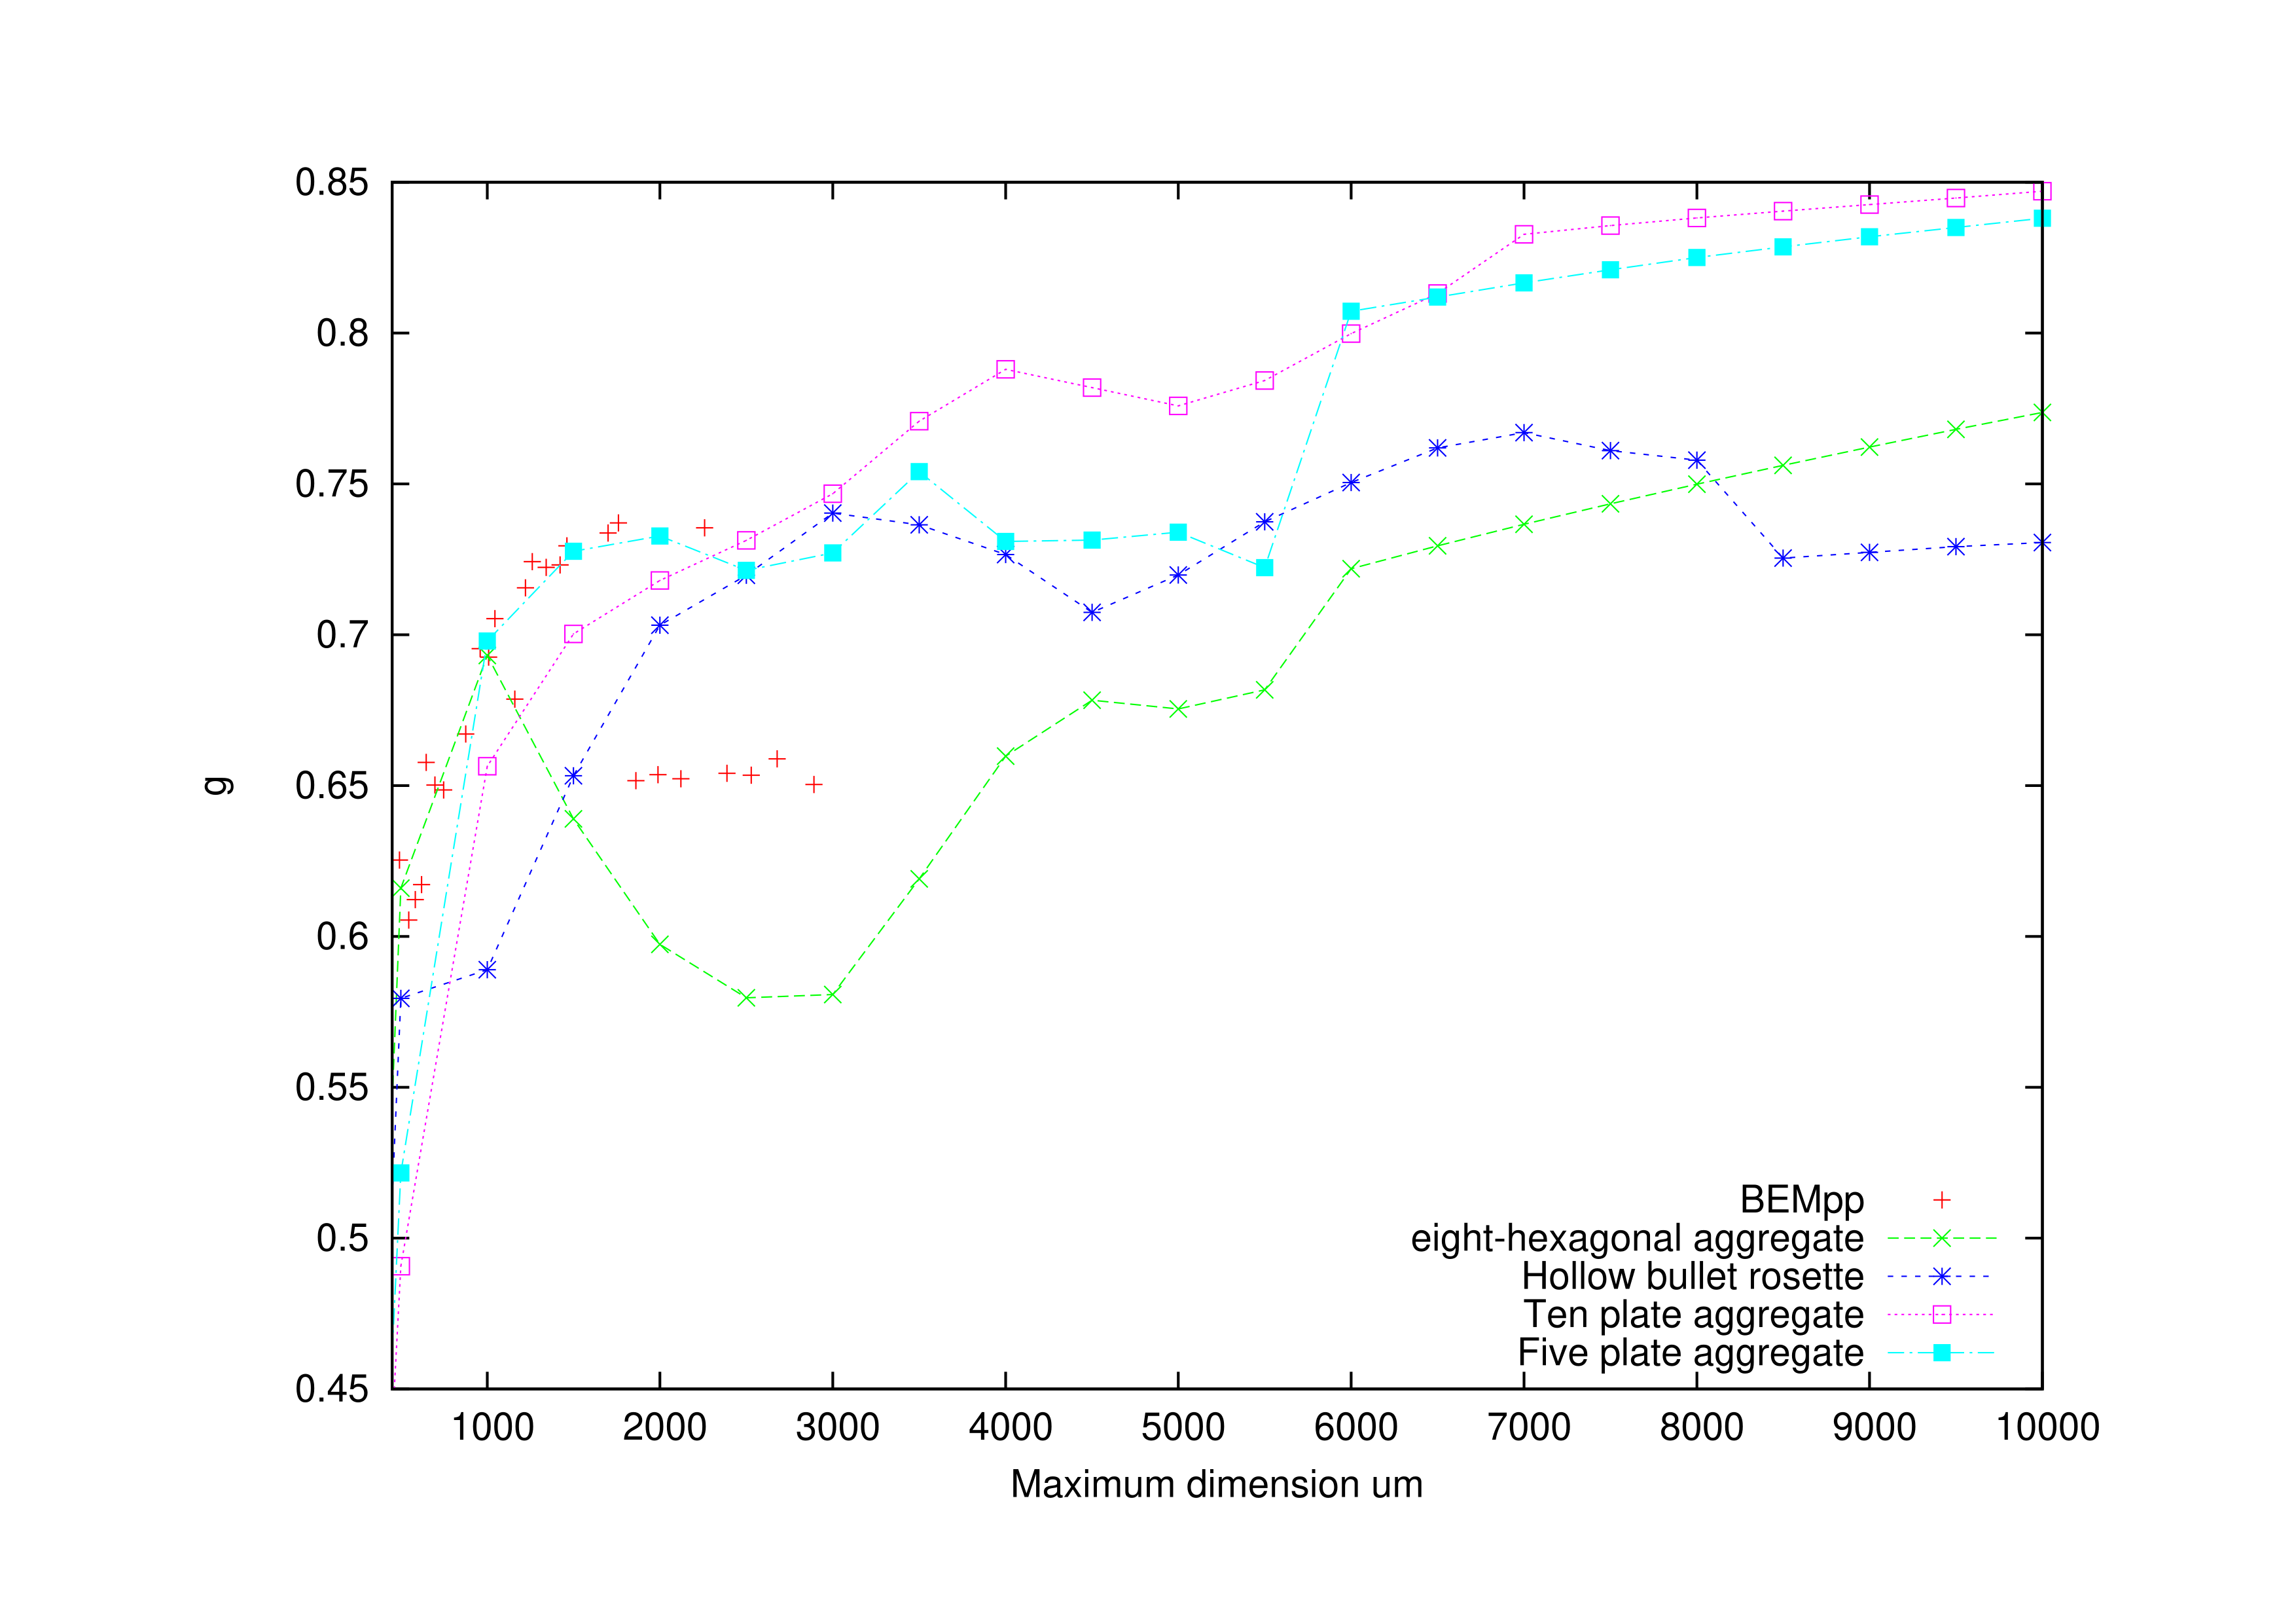
\includegraphics[width = 0.49 \textwidth]{Figures/rosette_aggregate_664ghz_tc_190_yang_g.png}
        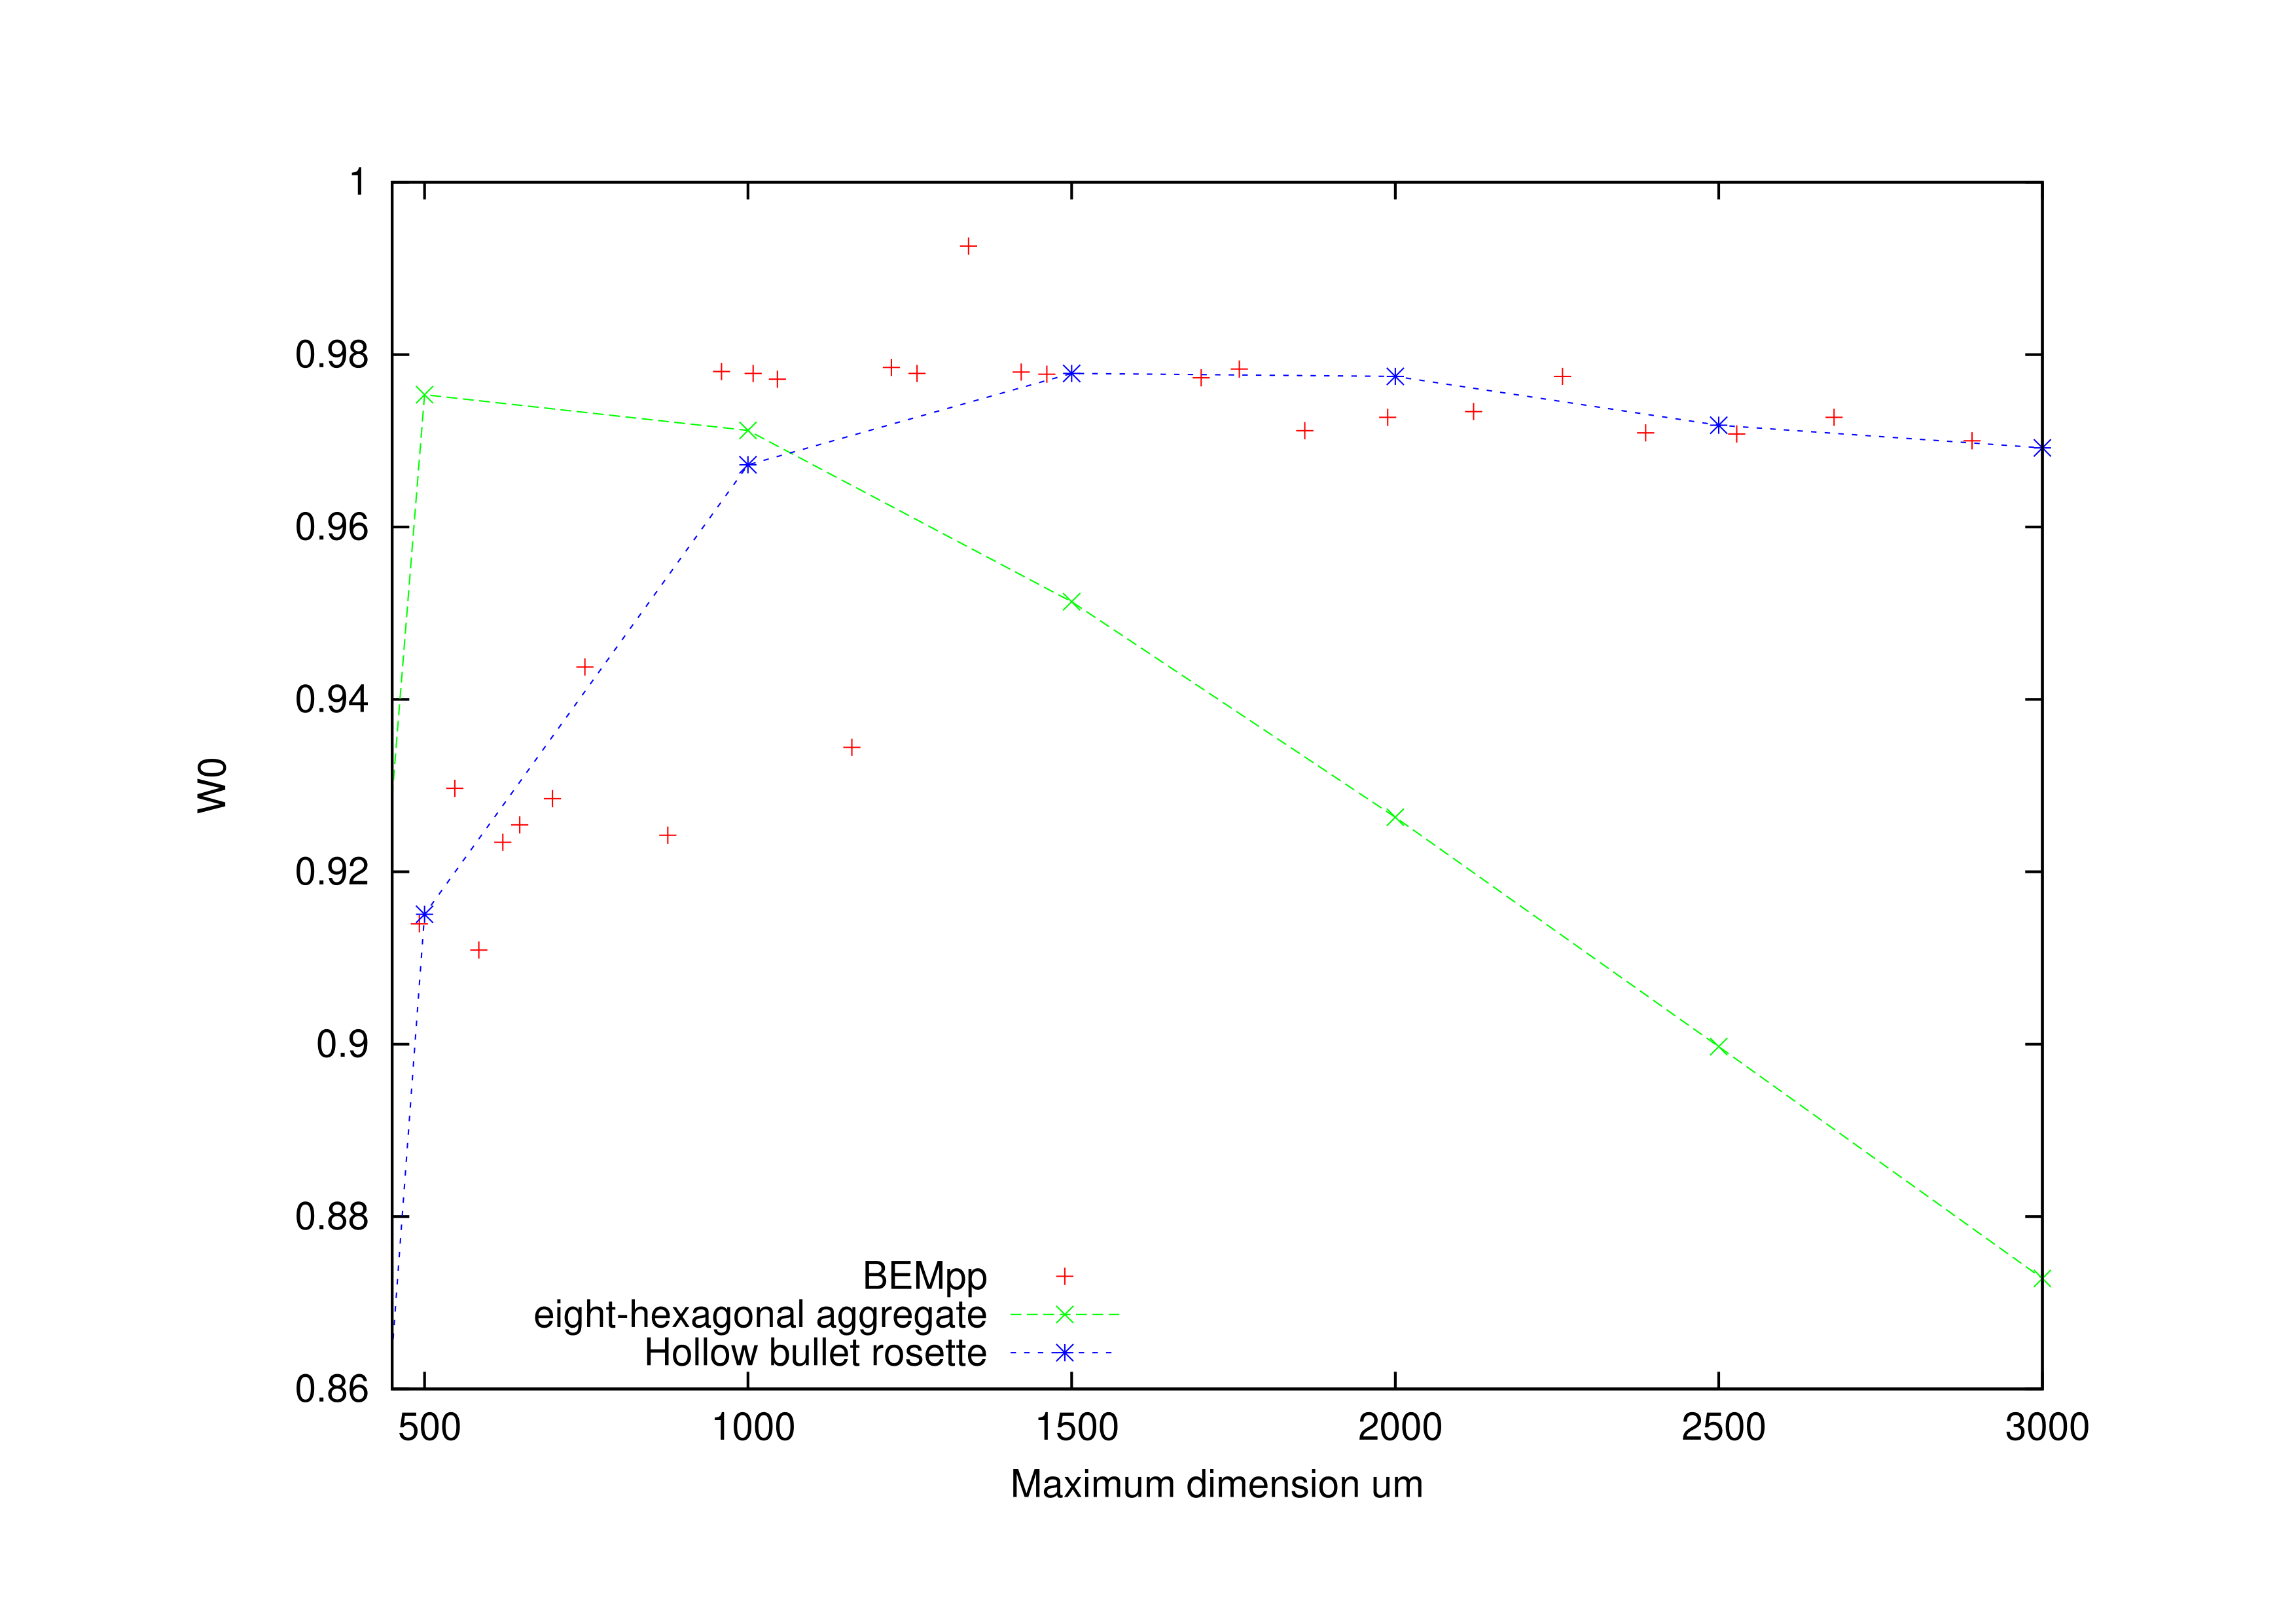
\includegraphics[width = 0.49 \textwidth]{Figures/rosette_aggregate_664ghz_tc_190_yang_w0.png}
    \end{figure}
\end{frame}
%%%

%%%
\begin{frame}{Current stage}
    \begin{itemize}
        \item Deployed the code on AWS (64 particle sizes, 5 temperatures, 4 frequencies)
        \item database to be delivered by 31st March 2020
        \item results for intermediate range particles for 664GHz, 243GHz and 183GHz
    \end{itemize}
\end{frame}
%%%
\end{document}

